% \documentclass[12pt]{scrreprt}
\documentclass[12pt]{report} 
% \documentclass[12pt, draft]{report} 

% language may be romanian or english (default is english)
% type may be bachelor or master (default is bachelor)
\usepackage[language=english, type=bachelor]{style}

%\geometry{a4paper,top=2.5cm,left=3cm,right=2.5cm,bottom=2.5cm}
%in style
%controlling the appearance of your headers and footers
\usepackage{fancyhdr}
\usepackage{amsfonts}
\usepackage{tabularx}
\usepackage{todonotes}
\usepackage{ltablex}
\usepackage{subcaption}
\usepackage{svg}
\usepackage[utf8]{inputenc}
\pagestyle{fancy}
\lhead{}
\chead{}
\renewcommand{\headrulewidth}{0.2pt}
\renewcommand{\footrulewidth}{0.2pt}

\begin{document}

\specialization{COMPUTER SCIENCE}
\title{Providing real-time information on mobile devices, using Progressive Web Apps}
\author{Pricop Laurențiu}
\supervisor{Lect. Dr. Dana Lupșa}

\maketitle

\newpage
\thispagestyle{empty}
\mbox{}
\newpage
\pagenumbering{roman}

\cleardoublepage
ABSTRACT
\vspace{0.5cm}
\hrule
\vspace{0.5cm}

Mobile devices are ubiquitous in the twenty-first century, and developing applications that work on them becomes ever harder and more complex, with more and more options for development. In this paper, we explore a particular method of developing mobile applications, that of the Progressive Web App (PWA), by creating a companion application for train trips.

In chapter one, we create an introduction of the subject, with some context in and around the theme, an outline of the goals of this thesis and related work.

In chapter two, we discuss at large the evolution of PWAs and how they trace back to the earliest computers, outlining the more important evolution milestones that shaped web applications into what they are today, providing comparisons between all applicable mobile architectures.

In chapter three, we outline a product design for our Train Companion application. We define the functionality, architecture, databases, components, and frameworks, while also talking about how we source the travel data.

In chapter four, we detail how this application was implemented, in relation to each point in the design. We discuss at large about different functionalities of the application, and detail the steps taken to enable PWA compliance.

In chapter 5, we provide a conclusion related to PWAs, and present in what ways they are better than native applications and in what ways they're worse.

\tableofcontents


\newpage
\pagenumbering{arabic}

\chapter{Introduction}

% Introduction: the paper's objectives and short description of chapters, overview of theme, highlight of personal contribution versus original results, and mention (if applicable) of the communication session where it was presented or the journal where it was published.

\section{Smartphones are everywhere}

The smartphone has seen an incredible rise in ubiquity since its inception. What could once be done only with an expensive desktop computer with a multitude of peripherals, is now available on a comparatively cheap mobile device.

Plotting market shares of desktop, mobile and tablet devices against one another, like shown in figure \ref{FigStatCounterDMT}, it is easy to notice how mobile devices have slowly overtaken desktop devices in popularity in the last 15 years.

\begin{figure}[htbp]
    \centering
    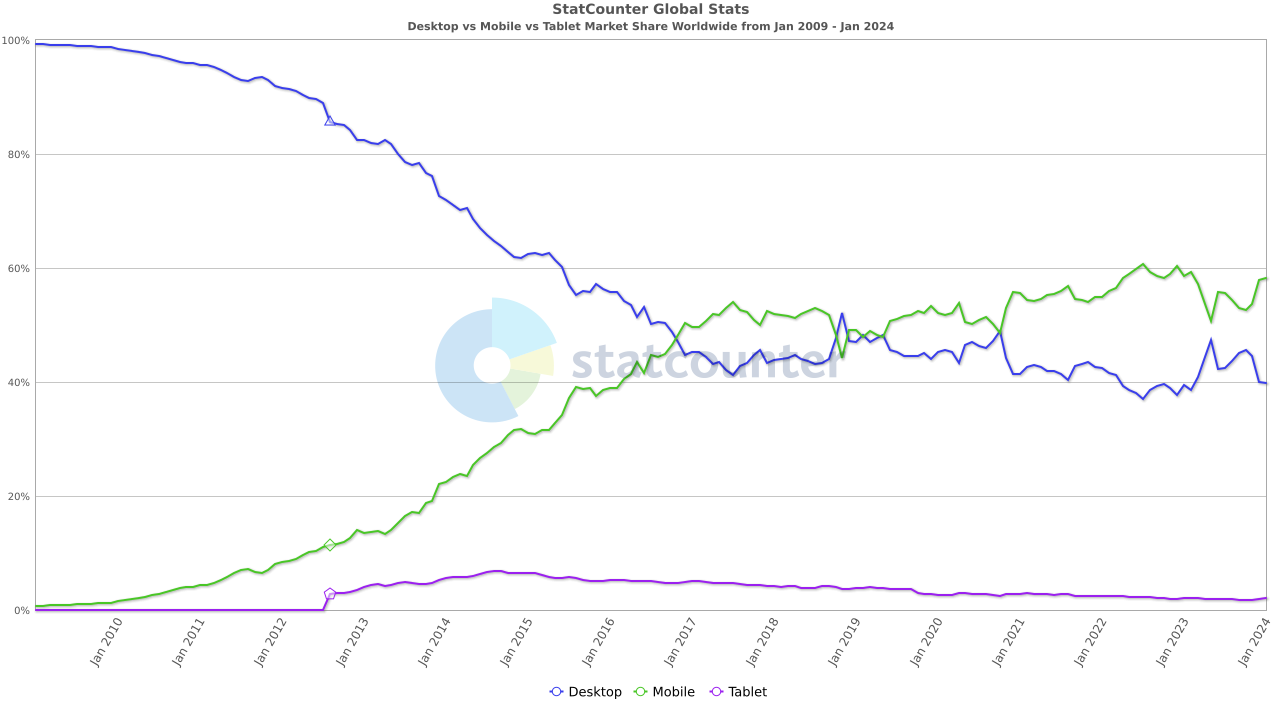
\includegraphics[width=\textwidth]{./figures/ch1_desktop-vs-mobile.png}
    \caption{Market shares of desktop, mobile and tablet devices, from January 2009 to January 2024 \cite{StatCountDMT}. Starting August 1st 2012, the chart counts tablets as a separate metric.}
    \label{FigStatCounterDMT}
\end{figure}

The trend of owning a mobile device shows that people prefer carrying a small and capable device around, rather than only being able to connect to the Internet using their fixed and comparatively large desktop device.

\section{Design differences and similarities between desktop and mobile}

\subsection{Evolution of desktop devices}

It is worth noticing that these two platforms could not be more similar to one another, yet have so many differences. Desktop devices have a notably different evolutionary tree to mobile devices, which means that not only do their shapes and buttons differ, but also their design philosophies.

Computers in their earliest forms were generally thought of as "boiler-room infrastructure" rather than personal devices. The advent of devices like the Apple II and software like VisiCalc, which was an advanced-for-the-time spreadsheet processor released in 1979, started to prove to the world that computers are not only useful when used by a trained team of experts, but can automatize tasks in the reach of a single employee. \cite{NYBirthPC}

These flashy, almost magical machines were starting to be capable of doing various tasks, from boring data processing to running graphics and games. This, combined with how they started to become more and more affordable, resulted in a boom in personal computer ownership starting in the 1980s.

\begin{figure}[htbp]
    \centering
    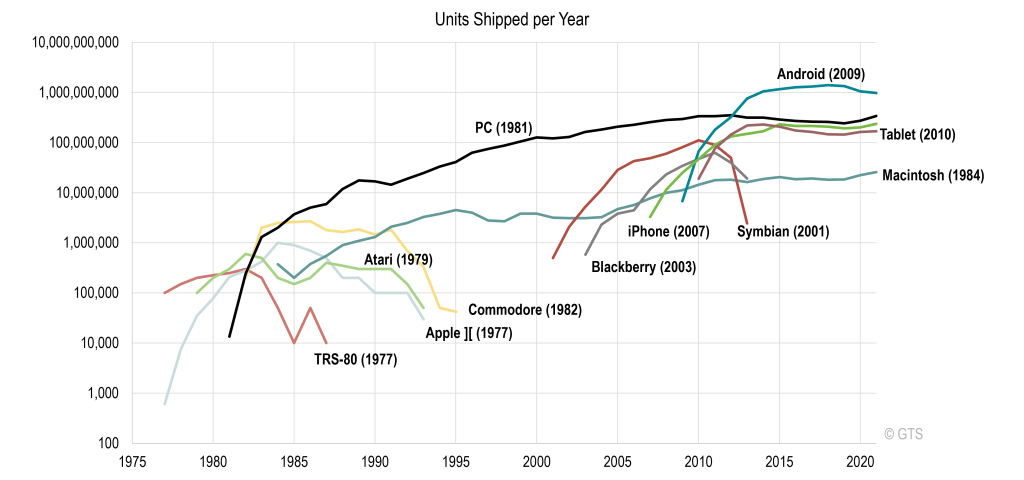
\includegraphics[width=\textwidth]{./figures/historical_pc_usage.png}
    \caption{Units Shipped per year for various desktop PCs and mobile devices, from 1977 to 2021. \cite{TGPCHis}}
    \label{FigHistoricalPC}
\end{figure}

This direct lineage between the personal computer and pre-1970 mainframes is apparent in the architectures of common operating systems like Windows or Unix. Given how specialized machines, that required trained people to use, started to spread to less technically advanced end-users, it is understandable that computer and operating system vendors tried to simplify how their systems were used.

In particular, the Personal Computer (PC) developed by IBM has seen the longest lifetime of a single lineage of computers \cite{TGPCHis}, being traceable all the way from 1981 to today. This suggests that the evolution of the IBM PC occurred in incremental steps, and to avoid having software vendors be forced to upgrade their software upon release of every version, it is understandable that IBM offered a degree of backwards compatibility.

As a result, design decisions that made sense in the 1980s started to be less useful.


\chapter{Evolution of PWAs. Capabilities. Comparison}

\section{Smartphones are everywhere}

The smartphone has seen an incredible rise in ubiquity since its inception. What could once be done only with an expensive desktop computer with a multitude of peripherals, is now available on a comparatively cheap mobile device.

Plotting market shares of desktop, mobile and tablet devices against one another, like shown in Figure \ref{FigStatCounterDMT}, it is easy to notice how mobile devices have slowly overtaken desktop devices in popularity in the last 15 years.

\begin{figure}[htbp]
    \centering
    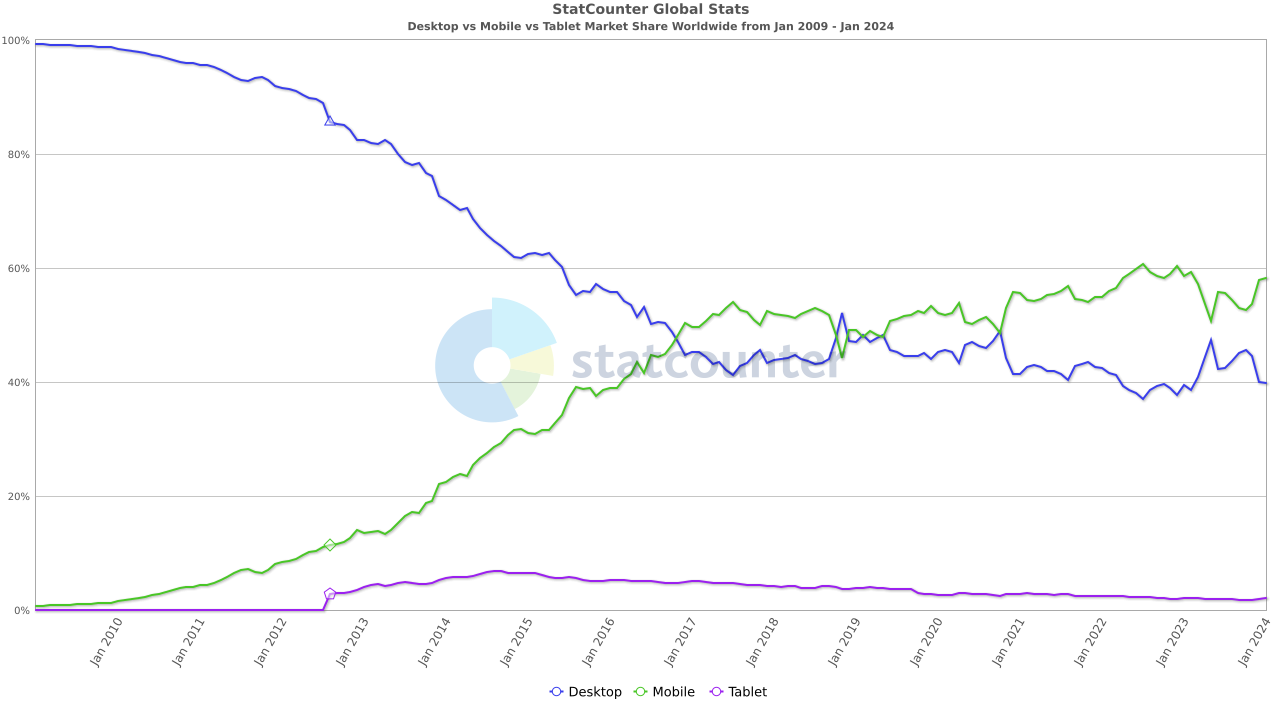
\includegraphics[width=\textwidth]{./figures/ch2_desktop-vs-mobile.png}
    \caption{Market shares of desktop, mobile and tablet devices, from January 2009 to January 2024 \cite{StatCountDMT}. Starting August 1st 2012, the chart counts tablets as a separate metric.}
    \label{FigStatCounterDMT}
\end{figure}

The trend of owning a mobile device shows that people prefer carrying a small and capable device around, rather than only being able to connect to the Internet using their fixed and comparatively large desktop device.

\section{Design differences and similarities between desktop and mobile}

\subsection{Evolution of desktop devices}

It is worth noticing that these two platforms could not be more similar to one another, yet have so many differences. Desktop devices have a notably different evolutionary tree to mobile devices, which means that not only do their shapes and buttons differ, but also their design philosophies.

Computers in their earliest forms were generally thought of as "boiler-room infrastructure" rather than personal devices. The advent of devices like the Apple II and software like VisiCalc, which was an advanced-for-the-time spreadsheet processor released in 1979, started to prove to the world that computers are not only useful when used by a trained team of experts, but can automatize tasks in the reach of a single employee \cite{NYBirthPC}.

These flashy, almost magical machines were starting to be capable of doing various tasks, from boring data processing to running graphics and games. This, combined with how they started to become more and more affordable, resulted in a boom in personal computer ownership starting in the 1980s.

\begin{figure}[htbp]
    \centering
    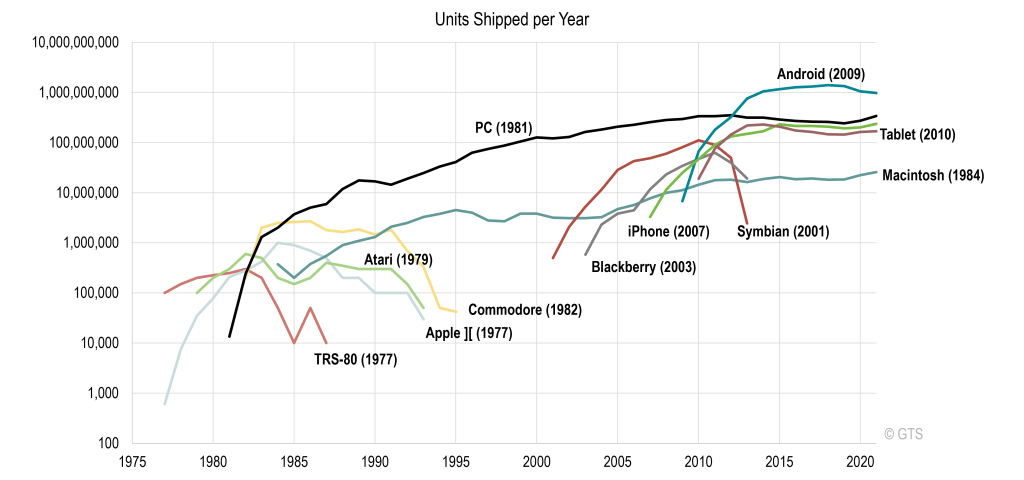
\includegraphics[width=\textwidth]{./figures/ch2_historical_pc_usage.png}
    \caption{Units Shipped per year for various desktop PCs and mobile devices, from 1977 to 2021 \cite{TGPCHis}.}
    \label{FigHistoricalPC}
\end{figure}

This direct lineage between the personal computer and pre-1970 mainframes is apparent in the architectures of common operating systems like Windows or Unix. Given how specialized machines, that required trained people to use, started to spread to less technically advanced end-users, it is understandable that computer and operating system vendors tried to simplify how their systems were used.

In particular, the Personal Computer (PC) developed by IBM has seen the longest lifetime of a single lineage of computers (Figure \ref{FigHistoricalPC}), being traceable all the way from 1981 to today. This shows that the evolution of the IBM PC occurred in incremental steps, and to avoid having software vendors be forced to upgrade their software upon release of every version, it is understandable that IBM offered a degree of backwards compatibility.

As a result, design decisions that made sense in the 1980s started to be less useful. A notable example of such design decisions can be found in modern Windows operating systems. The Microsoft documentation \cite{MSDNFolderNaming} has a clause that specifies a number of disallowed directory and file names, the likes of "CON", "PRN", "NUL", "AUX", and others, in addition to any combination of these names with any extension. This is very likely a result of the desire to keep backwards compatibility with old MS-DOS systems, that Windows can be directly traced to, which used these names as aliases for device drivers \cite{HusseinDeviceDrivers}.

\subsection{Evolution of mobile devices}
In comparison, the evolution of mobile devices and smartphones is very distinct and contained in a much shorter period of time.

The first device that was described as "the first time someone created a computer into the shape of a phone" is credited to be the IBM Simon, released around 1992. Boasting a touch screen and being portable, it had features such as a calculator and email. It has been described, retroactively, as "[being] the first smartphone. Twenty years ago, it envisioned our app-happy mobile lives, squeezing the features of a cell phone, pager, fax machine, and computer into an 18-ounce black brick"
\cite{SagerIraHistoryOfPhones}.

The year 1992 is very recent, compared to when the first computers started to become mainstream. This allowed phone manufacturers and OS vendors to learn from the mistakes done by personal computers, or optimize certain user experience facets.

An important step in the evolution of mobile devices is widely regarded as being the first iPhone. The hype Apple created about their new and flashy smartphone, culminating in around 11.000 print articles and 69 million hits on Google, seems to have been justified, and the phone was revolutionary, although somewhat flawed \cite{NYTAppleIPhoneRelease}. The iPhone defined a new era of smartphones, and many phone manufacturers have followed in the path that Apple laid out.

One of the core ideals of the iPhone is the ease of use. People that are non-technical find the iPhone accessible, and the way it seamlessly integrates with other Apple (sadly, only Apple) products proves that technology does not necessarily have to be hard to use \cite{SlashGearIPhoneOverAndroid}.

This trend manifests itself across the entire range of available mobile devices versus personal computers. Mobile phones are more widespread and are generally easier to use, having more friendly user interfaces and abstracting away hard technical details as much as possible.

\section{Native applications}

Mobile devices present ways of installing additional programs called "applications" that can extend the functionality of the device. Applications have proven to be the de-facto standard for implementing mobile functionality, and an ever-increasing number of companies offer their services through the apps that they constantly ask consumers to install.

From an architectural standpoint, these applications are strongly tied to the operating system architecture, and are therefore not portable.

\subsection{Architecture incompatibilities}

Having said that, an attempt at portability and standardization across mobile devices can be found within the Android Open Source Project (AOSP). An initiative by Google, the project offers a full mobile operating system under an open-source license, thus allowing any phone maker across the world to use it as a starting point for their own operating system.

While the AOSP initiative was a success and today many mobile devices have their roots in Android, phone manufacturers took to their own in creating an operating system with their own modifications, which make the Android ecosystem somewhat incompatible with itself, and lead to fragmentation of the Android market.

\begin{figure}[htbp]
    \centering
    \begin{subfigure}{.5\textwidth}
        \centering
        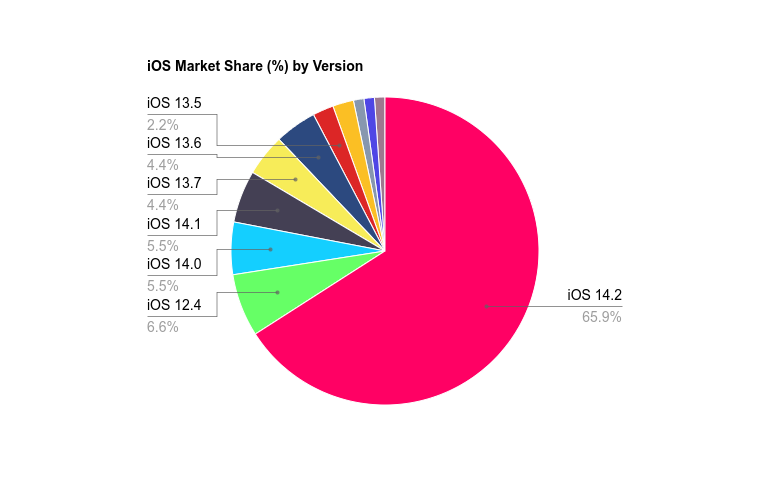
\includegraphics[width=\textwidth]{./figures/ch2_ios-market-share.png}
        \caption{iOS Market Share (\%)}
        \label{fig:sub1}
    \end{subfigure}%
    \begin{subfigure}{.5\textwidth}
        \centering
        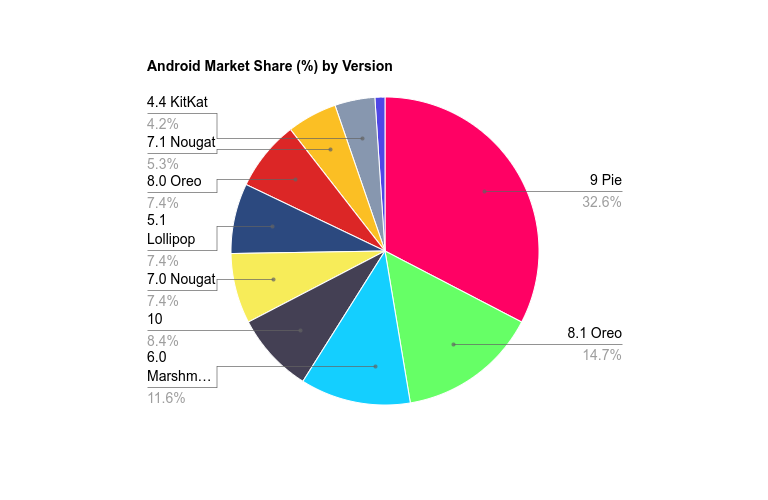
\includegraphics[width=\textwidth]{./figures/ch2_android-market-share.png}
        \caption{Android Market Share (\%)}
        \label{fig:sub2}
    \end{subfigure}
    \caption{Global market share of iOS versions, compared to Android versions \cite{StatCounterIOSVersionsMarketShare} \cite{XDADevsAndroidVersionsMarketShare}.}
    \label{FigAndroidVsIosFragmentation}
\end{figure}

A comparison between the Android and iOS ecosystems, with the former based on the AOSP project and the latter a proprietary system owned by Apple, presented in figure \ref{FigAndroidVsIosFragmentation}, shows the striking difference between the market shares of the respective latest versions. The Android market fragmentation can be attributed indirectly to its open-source model, and is in direct contrast with the proprietary model of Apple and its control over the entire iOS ecosystem.

This is but one example of the incompatibilities of native application across mobile device operating systems. Generally, developing an application that is desired to reach as many users as possible requires developing for a range of architectures, such as iOS, Android or Huawei.

\subsection{Ecosystem control}
Distribution of native applications is generally done using application marketplaces that are proprietary to each phone manufacturer. Examples of such marketplaces include Google's Play Store, Apple's App Store, or Huawei's AppGallery. These marketplaces provide services such as automatic updates and ability to review apps.

However, these marketplaces also represent a way of controlling the application ecosystem. One marketplace known for very carefully curating apps in its distribution system is Apple's App Store.

Apple imposes very strict rules on its applications, aiming to preserve their users' privacy and experience. As an example, they restrict access to device sensors that can be used for user fingerprinting, and require justification if a sensor is requested by an application \cite{ZdnetNewAppleStoreRules}.

This being said however, it is also worth mentioning that Apple takes a commission of all sales performed through its App Store (store purchases, in-app purchases) that can reach percents of 30\%. These high profits have the potential to justify some other market manipulation tactics that Apple employs.

Apple is known to handle Internet browsing on iOS in ways that can be considered a way of market manipulation. Instead of offering alternatives to their high-commission marketplace, they intentionally avoid implementing important Web APIs in their proprietary WebKit browser engine used by Safari \cite{ZdnetAppleDeclinedWebApis}, while not allowing, as per App Store policy, alternative browser engines \cite{AppleGuidelinesWebkit} (note that regulations in the European Union might force Apple to provide limited support for such alternatives \cite{AppleAlternativeBrowsersEU}).

Apple's reasoning for not implementing Web APIs relating to phone sensors and telemetry (NFC, battery, bluetooth, geo-location) is that they value users' privacy, even though these APIs are not that related to privacy but rather to an application's ability to get shipped as a Web app rather than a native, App Store app.

\subsection{Device access}
By nature of being specifically built for the target architecture, native applications have an unmatched capability of making use of the phone hardware. Having no additional layers between application code and operating system (e.g. a browser runtime and sandbox), native code has access to all the operating system system calls exposed to native applications, and can also achieve unmatched runtime performance.

% \section{Hybrid (cross-platform interpreted) applications}

\section{Web applications}
Even in the early days of the Internet, rudimentary forms of websites, that can be called web applications, existed. One of the pioneering frameworks for creating such interactive experiences begun as the Personal Home Page programming language, also known as PHP, released around 1995. It had the ability to render dynamic pages and handle user forms, which already compose a functional web application. Over the years, PHP has grown in popularity and it has got incremental updates, such that it now powers over 70\% of the websites on the Internet \cite{TurnkeyPHPIsNotDead}. It envisioned having web applications work in a simple "request page $\rightarrow$ response with page" model (figure \ref{FigPHPSeqDiag}).

\begin{figure}[htbp]
    \centering
    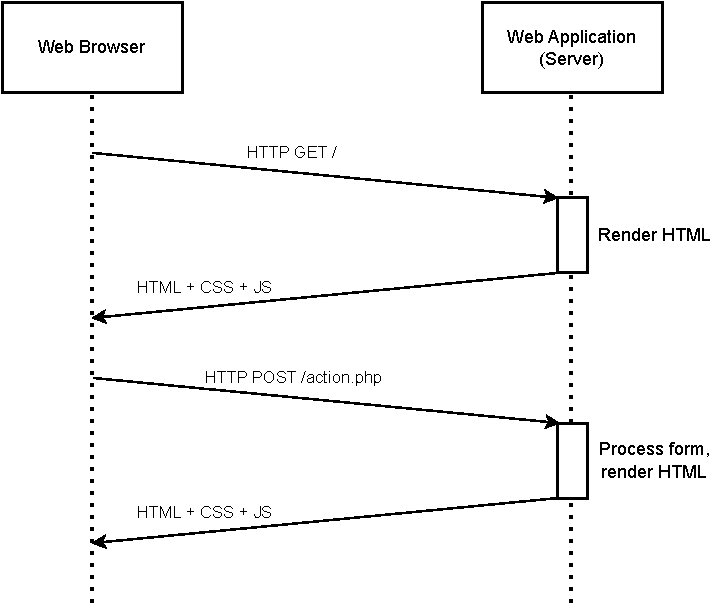
\includegraphics[width=0.7\textwidth]{./figures/ch2_php-seq-diag.pdf}
    \caption{Illustrative diagram of how a PHP-based website might process requests.}
    \label{FigPHPSeqDiag}
\end{figure}

An important step in the evolution of dynamic web pages was the introduction of AJAX around the year 2005 \cite{PWAShortHist}. AJAX, short for Asynchronous JavaScript and XML, enabled web pages to make additional HTTP requests initiated by client-side JavaScript code. These asynchronous HTTP requests could then be used to dynamically update contents of the page, without needing a full page refresh (figure \ref{FigAJAXSeqDiag}). However, a backend server that can generate HTML code was needed to render the initial page, even if subsequent AJAX requests didn't transfer information in HTML representation (ie. JSON).

\begin{figure}[htbp]
    \centering
    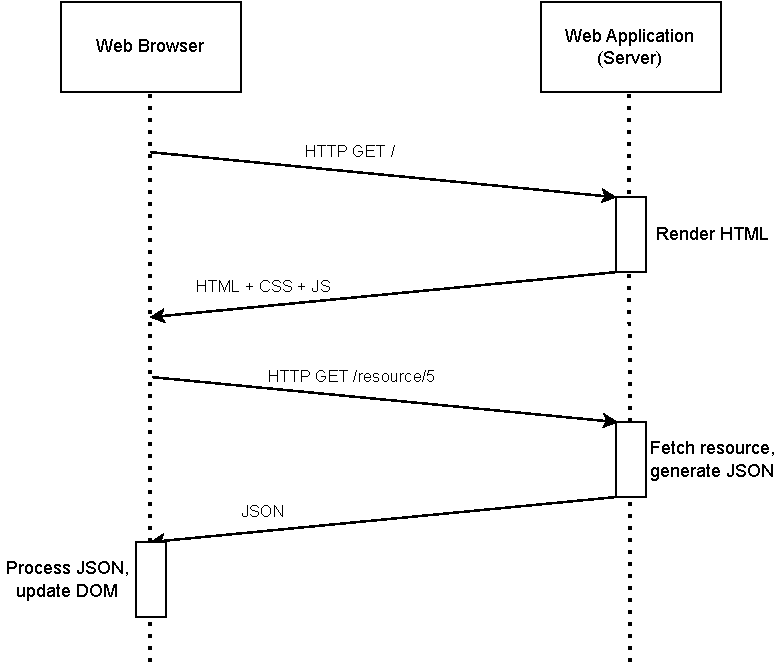
\includegraphics[width=0.7\textwidth]{./figures/ch2_ajax-seq-diag.pdf}
    \caption{Illustrative diagram of how a website making use of AJAX calls might process requests.}
    \label{FigAJAXSeqDiag}
\end{figure}

Incremental improvements in the JavaScript standards, and new and novel frontend frameworks that attempted to ease the injection of \( f(state) \Rightarrow view \) (such as React, Angular) enabled a new form of web application to take shape: that of the Single Page Application.

The Single Page Application enabled separating an application into two completely separate components: a backend and a frontend. For the first time, backends could expose some endpoints, collectively called an API, that then the frontend could use to communicate with the backend (figure \ref{FigSPASeqDiag}). This separation enabled the frontend to be easily shipped as a static site across the world, the backend to become extremely simple and only communicate using JSON/XML, and so much more.

\begin{figure}[htbp]
    \centering
    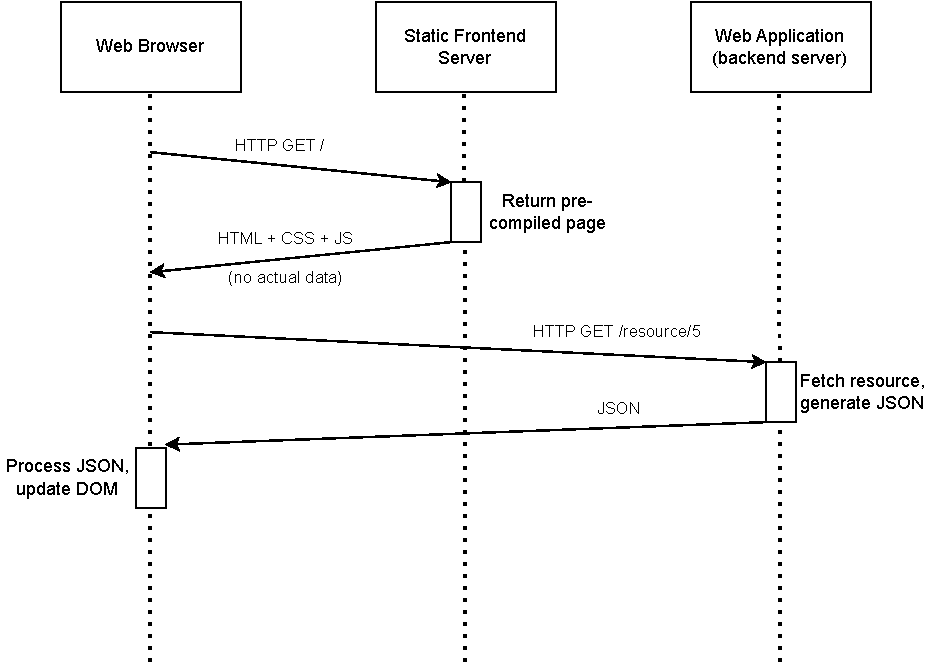
\includegraphics[width=0.85\textwidth]{./figures/ch2_spa-seq-diag.pdf}
    \caption{Illustrative diagram of how an application with separate backend and frontend might process requests.}
    \label{FigSPASeqDiag}
\end{figure}

\subsection{Browser inconsistencies}

Although in a much better state nowadays, browsers often preferentially implement certain Web APIs, creating many subtle incompatibilities between browser vendors. Tools like "Can I use" \cite{CanIUse} are the first thing a web developer checks for whenever they want to use a more obscure Web API.

However, API and engine differences have historically been mitigated by use of polyfills. Tools like Babel or TypeScript can also aid by providing a build step to JavaScript code that can transform the code to automatically enable support for various JavaScript standards.

Additionally, minor visual inconsistencies can also occur within the same brow\-ser vendor. Users might have different font sets installed, different screen sizes, or use browser functionalities that alter the page, like zoom, reader mode, etc.

\subsection{Browser sandbox}
All web applications that run in a browser are subject to the sandbox that the brow\-ser confines the JavaScript code within. Web applications can only access device capabilities that the browser provides access through, and can only do so reliably if they are covered by a standardized Web API.

This can understandably apply limitations to what an application shipped using the Web can do.

\subsection{Decentralized distribution}
Web applications are always distributed to users by means of the Internet. This means that there exists no single authority that can veto the distribution of certain applications, unlike the mobile marketplaces mentioned above.

Additionally, by nature, web applications are always kept up-to-date. They are downloaded on-demand, meaning that updates can be transparently and easily pushed to users. Even if the frontend is cached on the end-users' devices, the developers can be sure that setting a certain cache validity period means that no user will have the old version of the app once that validity period expires.

\subsection{The step towards PWA}

It is worth noticing that the "static frontend" component shown in figure \ref{FigSPASeqDiag} can be treated in a language-agnostic way. The frontend can easily be written using any frameworks or languages of preference (React, Angular, Vue; JavaScript, PyScript, compiled WebAssembly), without needing to alter in any way the backend infrastructure. In fact, we need not be constrained by something that can run in a browser: this frontend can even take the form of a mobile application.

We have already examined mobile applications, so it is time to explore a way to bring out the best of both worlds, using Progressive Web Apps.

\section{Progressive Web Apps}

Progressive Web Apps are not a concrete technology, but rather a collection of features that an app offers such that it can integrate with the browser and informs it that it possesses the qualities of a PWA.

The basis of a PWA is but a plain web application, namely a Single Page Application, that boasts a number of minor modifications and additions to make it suitable for offline functionality and local installation.

In the following chapters, we design and implement a React application with a tiny backend that makes use of different Web APIs such as live location and IndexedDB, while also offering PWA compliant functionality.
\chapter{Product design}

\section{The real-world problem}
The Romanian national railway operator, CFR S.A. is tasked with the upkeep of 20 thousand kilometers of un-electrified and electrified railway spread out over 9 main lines \cite{CFROrdinMagistrale} \cite{WallstreetRoReorganizareSNCFR}, stretching all across Romania.

\begin{figure}[htbp]
    \centering
    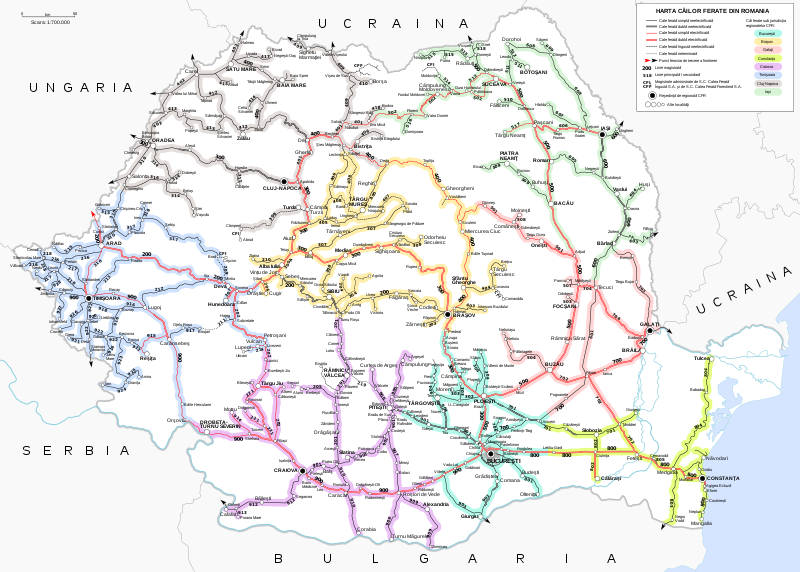
\includegraphics[width=0.8\textwidth]{./figures/ch3_romania-feroviara.png}
    \caption{Map of Romania's railway network. Map by Aero Avalon, shared under CC-BY 4.0 \cite{WikipediaRomaniaFeroviara}.}
    \label{FigRomaniaFeroviara}
\end{figure}

The passenger subsidiary, CFR Călători, is the biggest railway operator that makes use of these lines. However, rolling stock is outdated and most train cars lack modern features like driver-controlled doors. A notable absence though is that of live travel information offered inside the train to the passengers. An example of such an information display is given in Figure \ref{FigMAVInterior}.

\begin{figure}[htbp]
    \centering
    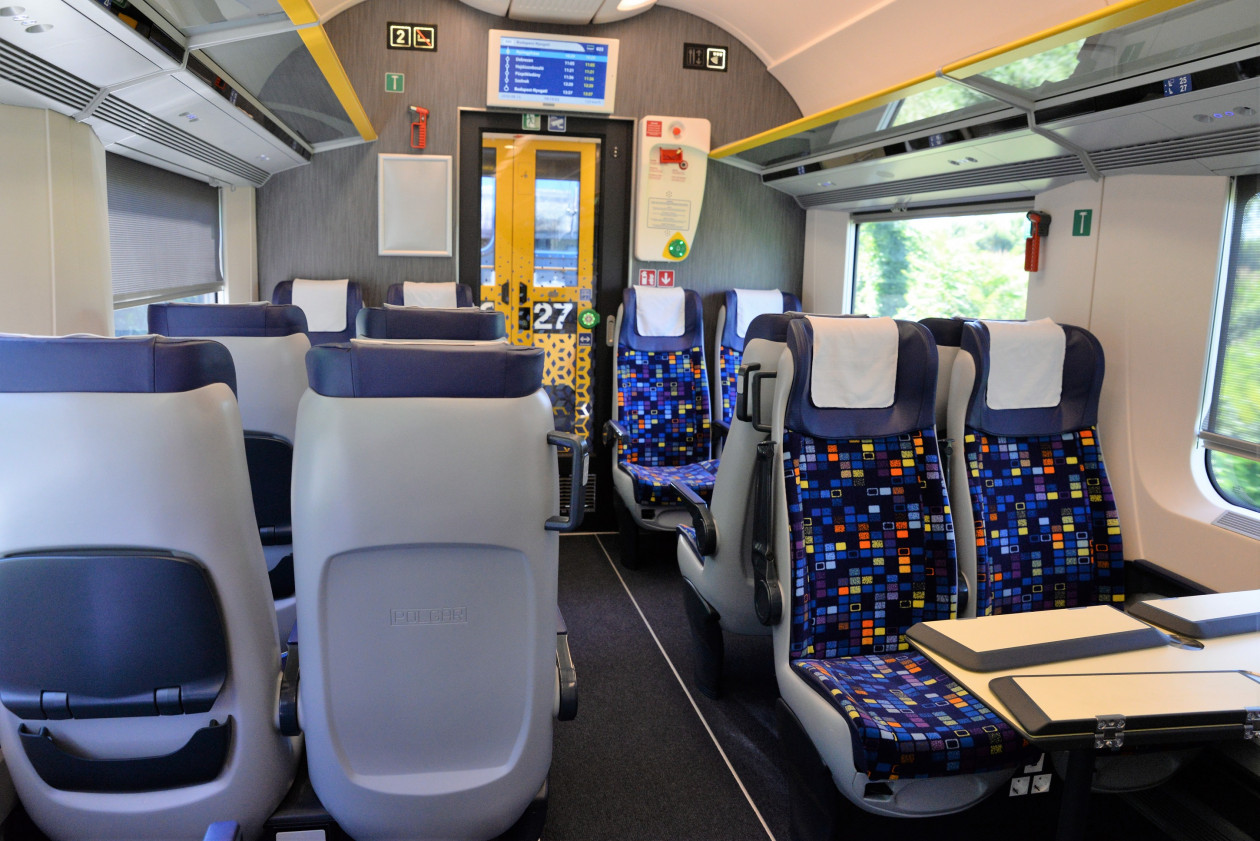
\includegraphics[width=0.8\textwidth]{./figures/ch1_mav-interior.png}
    \caption{Interior of a train owned by MÁV-Start, the Hungarian national passenger operator \cite{PestiHirlapMAVInterior}. The LCD display can be seen at the top, providing information about the next stations, times and delays. Stations and times can be pre-programmed into the train on departure, but delays require live integration with a central service.}
    \label{FigMAVInterior}
\end{figure}

Given that retrofitting all rolling stock with displays connected to the Internet is a challenging task, CFR Călători has attempted digitization in various other ways.

In 2016, the company launched IRIS, a web application that provided traffic information about the company's trains. It also offered information about delays \cite{StiriDeClujLansareCFRIris}. In 2018, IRIS got discontinued in favor of a newer platform, written in ASP.NET, which offers information about all railway operators in Romania.

In 2021, the company launched a mobile application with all the capabilities that the website has, making it more convenient than ever before to view traffic information \cite{MobilissimoCFRLansareMobil}.

These solutions, however, are insufficient in answering the question of "Where am I?" that a passenger might have. The most significant issue is that they all require Internet, the lack of which is an issue prevalent across Romanian trains \cite{CFRInternetIC}.

Moreover, CFR does not track the location of their trains using GPS transponders or any similar technology, but rather using personnel that are responsible with coordinating the trains passing through each station. This brings a number of issues:

\begin{itemize}
    \item \textbf{Data is not real-time.} A train passing through a station is only recorded when the station personnel manually records that train as passed, in the company's internal services.
    \item \textbf{Data might be missing.} Some personnel might not take the time to enter delay data for each passing train.
    \item \textbf{Some stations are not tracked.} Some train stations are big enough to be serviced by regional trains, but not big enough to warrant any personnel responsible with train movement.
    \item \textbf{Data might be false.} Station personnel can enter any delay data they want, having the possibility of hiding delays.
\end{itemize}

\section{Application requirements}
\label{sec:Requirements}

Given the set of real-world issues mentioned above, we can create a set of requirements for an application that tries to plug the information gap and provide a seamless travel experience for the passenger.

The basic idea of this thesis is to merge the mobile app experience and the website experience offered by CFR into a single solution, that will then be extended to offer live traffic information using phone capabilities such as the camera and location.

\begin{enumerate}
    \item Train trip information
          \begin{itemize}
              \item The app should allow the user to create a new trip. The user will be able to view live information about this trip.
              \item The app should be able to show details about the user's current position in their trip, using information obtained from user (train ticket), train database (itinerary of train) and phone sensors (GPS location).
              \item The live information should include: next stop, last stop, next stop arrival time (timetabled), train delay, next station of pass-through (if applicable).
              \item The live information may also include the destination arrival time (time\-tabled) + train delay.
              \item Information about the train ticket can be obtained using multiple methods: scanning the QR code of the ticket (state operator only), or manually inputting ticket data (train number, destination station).
              \item Access to non-live data should be provided via links to the Mersul Trenu\-rilor website (train itinerary, station stops).
              \item National train itinerary information will be saved to the user's device on application install. The information can be updated from the server. Attempts to automatically update this data will be done weekly.
          \end{itemize}
    \item User profile and authentication
          \begin{itemize}
              \item The app should be able to be used anonymously, without login. If so, persistent data must be saved locally to the device.
              \item The app must provide social login (login with Google, login with Apple) as the primary means of logging in.
              \item When creating a new account (logging in for the first time), if there is local data on the device, the app must offer the user the possibility of migrating it to the account. If logging into an existing account, local data must be deleted.
              \item The app must be able to show to the user a history of their trips.
              \item Logging in on another device will log out the already-logged-in device.
          \end{itemize}
    \item Connectivity
          \begin{itemize}
              \item The app must work without Internet, except for functionalities that directly require it.
              \item Account login will not work without Internet.
          \end{itemize}
          \item{Internationalization}
          \begin{itemize}
              \item The app must provide multi-language support (Romanian and English).
          \end{itemize}
\end{enumerate}

\section{Guiding principles}

To maximize user adoption and ease of use, the application should be centered about these core principles:

\begin{itemize}
    \item \textbf{Offline:} it will work at maximum capability while offline.
    \item \textbf{Easy to get into:} users should be able to get live tracking as soon as they click a link, and should not have to install apps.
    \item \textbf{Live information:} the screen will update as soon as the app gets new traffic or position information.
    \item \textbf{Information at a glance:} all information needed to answer the questions of "Where am I?", "How long until next stop?", "How long until my stop?" is always displayed on-screen.
    \item \textbf{Minimal configuration:} integrate with existing CFR services and ticketing systems as seamlessly as possible.
    \item \textbf{Avoid "yet another account and password":} allow the user to save their preferences locally, or use social login to sync them. Do not ask the user to remember another password!
\end{itemize}

\section{Use case diagram}

We can also design a use case diagram showing the main functionalities of the application and how we intend them to interoperate and operate with the various actors, in Figure \ref{FigUseCase}.

\begin{figure}[htbp]
    \centering
    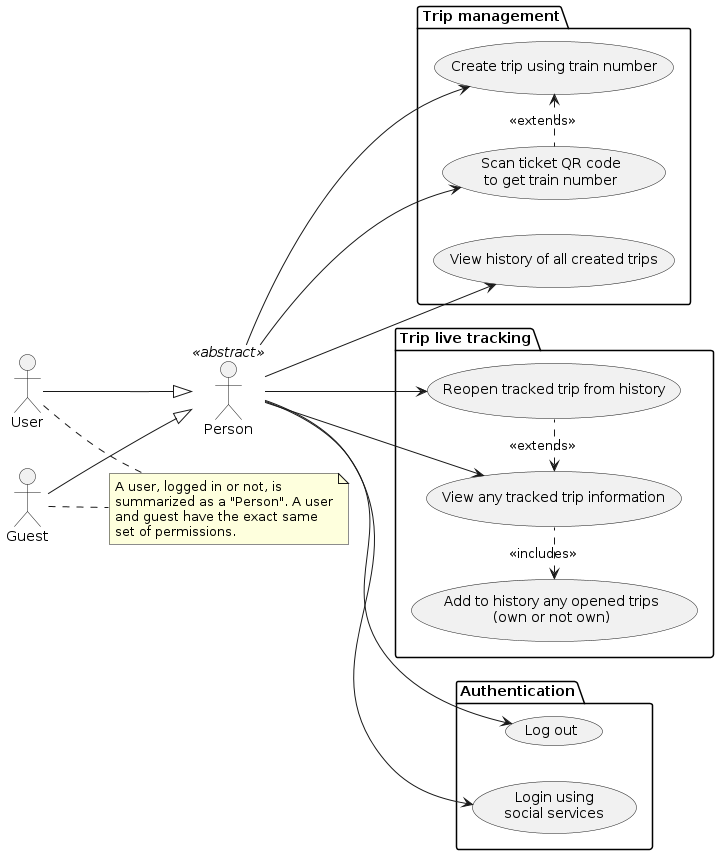
\includegraphics[width=0.9\textwidth]{./figures/ch3_use-case.png}
    \caption{Use case diagram for our CFR Companion application.}
    \label{FigUseCase}
\end{figure}

As you can see, even though we employ user accounts, there is little operational difference between users that are logged in, and those who are not. The permission set is the same, what is different is where the user data (trip history) is saved.

\iffalse
    \section{MOMENTARILY DISCARDED: User stories}

    Given the set of core principles outlined in the previous section, a list of user stories can be compiled. Features that are \textbf{not} necessary for a Minimum Viable Product (MVP) are marked as such and are de-prioritized.

    A minimum viable product, in our case, comprises the set of features needed to fullfil our core principles.

    I used the shorthand "AaU" to mean "As a User".

    \begin{tabularx}
        {\linewidth}{
            | >{\hsize=.15\hsize}X
            | >{\hsize=.65\hsize}X
            | >{\hsize=.2\hsize}X |
        }
        \hline
        Category / Story \# & User story                                                                                                           & Scope        \\
        \hline\hline
        \multicolumn{3}{|X|}{1. Live Location}                                                                                                                    \\
        \hline 1.1.         & AaU, I want to see live where I am, what's the next station, and when I get there                                    & MVP          \\
        \hline 1.2.         & AaU, I want to manually input my train number so that the app knows                                                  & MVP          \\
        \hline 1.3.         & AaU, I want to be able to make a picture of my ticket so that the app can figure out my train number                 & Nice to have \\
        \hline 1.4.         & AaU, I want to be able to scan the ticket's QR code so that the app can figure out my train number                   & Nice to have \\
        \hline 1.5.         & AaU, I want to send a screenshot of an online ticket (or the CFR PDF) so that the app can figure out my train number & Nice to have \\
        \hline 1.6.         & AaU, I want to see, live, what delay my train has                                                                    & MVP          \\
        \hline 1.7.         & AaU, I want to see, live, what the next and last stations are                                                        & MVP          \\
        \hline 1.8.         & AaU, I want to see intermediary stations where the train doesn't stop                                                & Nice to have \\
        \hline 1.9.         & AaU, I want to see, on a map, where I am                                                                             & Nice to have \\
        \hline 1.10.        & AaU, I want to see what station I get off at, and see when I get there                                               & Nice to have \\
        \hline
        \hline
        \multicolumn{3}{|X|}{2. Schedules Information}                                                                                                            \\
        \hline 2.1.         & AaU, I want to see, for a station, what trains arrive there, and at what times                                       & MVP          \\
        \hline 2.2.         & AaU, I want to see, for my train, all stations it has                                                                & MVP          \\
        \hline 2.3.         & AaU, I want to see, for my train, all intermediary stations that it does NOT stop at                                 & Nice to have \\
        \hline
        \hline
        \multicolumn{3}{|X|}{3. User profile and Authentication}                                                                                                  \\
        \hline 3.1.         & AaU, I want to be able to use the app anonymously                                                                    & MVP          \\
        \hline 3.2.         & AaU, if I create an account, I want to be able to merge my data into the account                                     & Nice to have \\
        \hline 3.3.         & AaU, I want to be able to register/login using my Apple account                                                      & MVP          \\
        \hline 3.4.         & AaU, I want to be able to register/login using my Google account                                                     & MVP          \\
        \hline 3.5.         & AaU, I want to be able to optionally set up 2FA using an Authenticator app                                           & Nice to have \\
        \hline 3.6.         & AaU, if I have 2FA on, I want to be able to login using a recovery code                                              & Nice to have \\
        \hline 3.7.         & AaU, I want to add a train trip to my history, manually                                                              & MVP          \\
        \hline 3.8.         & AaU, I want to have any ticket I scan added automatically to my history                                              & Nice to have \\
        \hline 3.9.         & AaU, I want to see the history of my train trips                                                                     & MVP          \\
        \hline 3.10.        & AaU, I want to see a digest of my history: most visited station, most traveled-on route, etc                         & MVP          \\
        \hline
        \hline
        \multicolumn{3}{|X|}{4. Internationalisation}                                                                                                             \\
        \hline 4.1.         & AaU, I want to be able to select a language I prefer to see the app in (EN / RO)                                     & MVP          \\
        \hline
        \hline
        \multicolumn{3}{|X|}{5. Appearance}                                                                                                                       \\
        \hline 5.1.         & AaU, I want to be able to select a dark or light theme                                                               & Nice to have \\
        \hline
    \end{tabularx}
\fi
\chapter{Application implementation}

\section{Backend server}

The backend server does not need to be particularly suited for large traffic or complexity. Its role is only to provide up-to-date GTFS data and manage user accounts. To this end, let's discuss about how it has been implemented.

As mentioned in the previous chapter, I used NestJS with TypeScript to build the backend server. NestJS is an opinionated framework that brings important abstractions (in the form of decorated classes and dependency injection) on top of an already-proven, battle-tested, HTTP server library (Express JS). NestJS can work with plain JavaScript, but augmenting it with TypeScript brings forth is fullest potential.

NestJS is heavily inspired from Angular, thus employs a system of \textit{modules}, that can be loaded into a Nest application individually, along with its dependencies, to the programmer's wish. Organizing into separate modules, or bundling everything into the default App module, is a decision taken by the programmer, taking into consideration applications such as microservices (different modules within the same project can be useful here) and complexity concerns (modules are hard to get to work). I chose to structure my project in modules that correspond to the following functionalities: authentication, GTFS file operation, user management.

\subsection{App module}
\label{sec:AppModule}

The App module is the big module that gets loaded and ran on application bootstrap. Presented in Figure \ref{FigBeBootstrap}, the application bootstrap code will initialize the Nest application using the \verb|AppModule| module as a root module, then takes some final steps in the setup of the environment, by disabling all CORS functionality and allowing all origins, allowing access to static assets (namely, the GTFS data, which is stored locally), and setting up the global \verb|ValidationPipe|, which takes care of request validation. When ready to listen to requests, we take the port from the environment (or use 3000 as default), then we start the Nest application.

\begin{figure}[htbp]
    \centering
    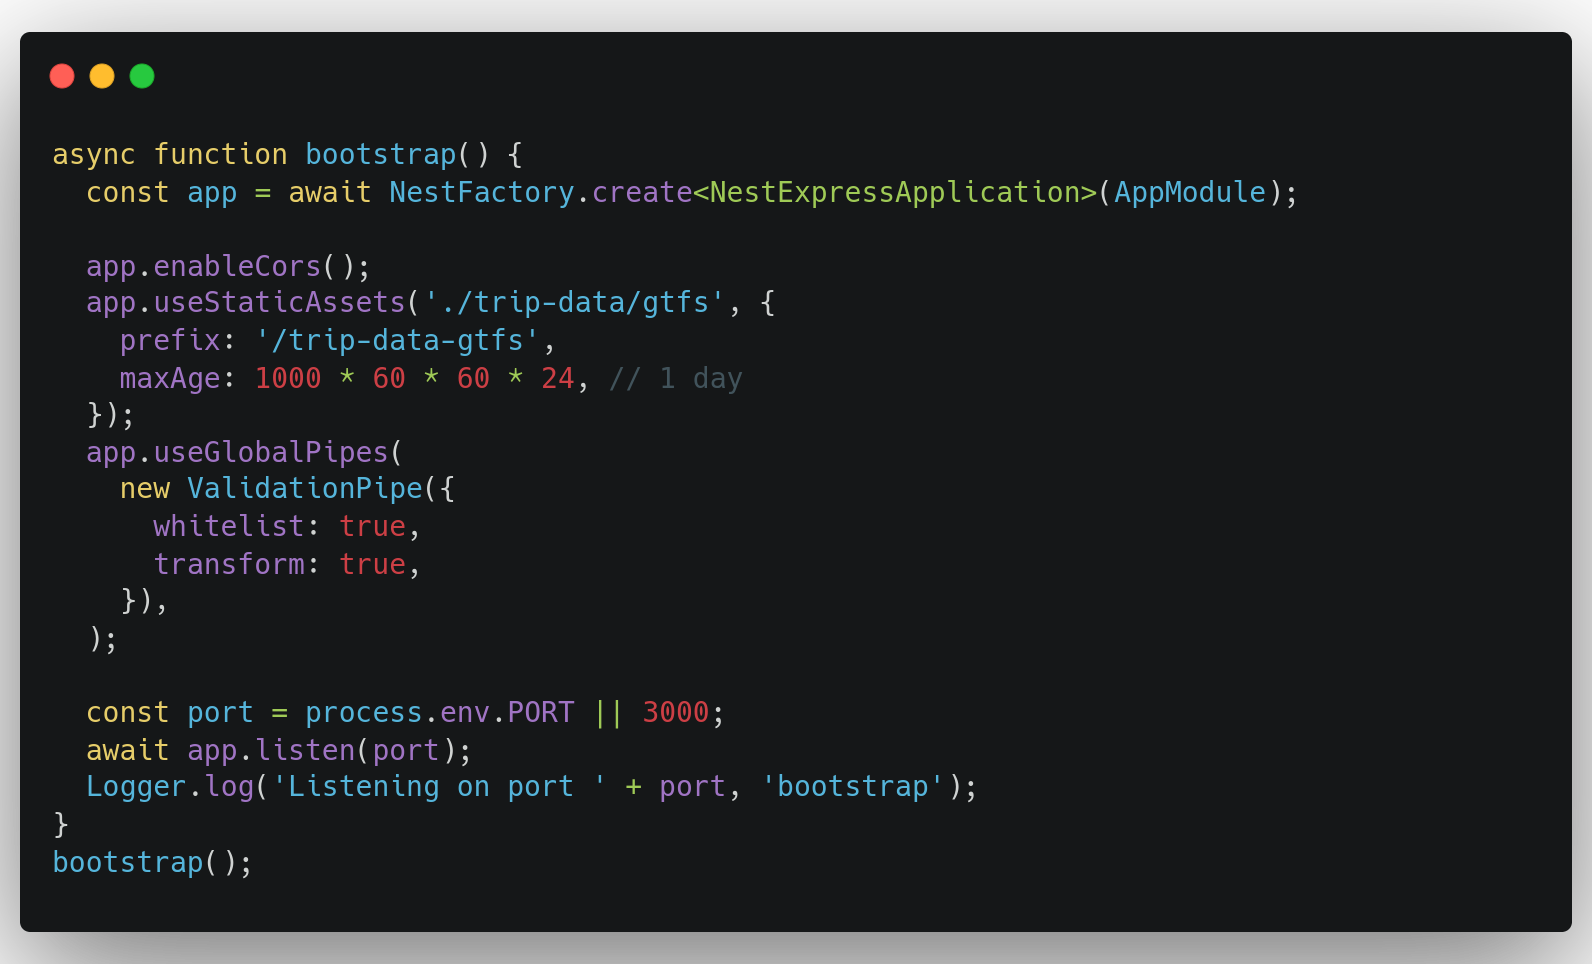
\includegraphics[width=0.9\textwidth]{./figures/code/be_bootstrap.png}
    \caption{Backend: bootstrapping code.}
    \label{FigBeBootstrap}
\end{figure}

Module definitions are not much more complex than importing all the dependency modules and adding them in the module definition, using the \verb|Module| decorator. The definition of the \verb|AppModule| is presented in Figure \ref{FigBeAppModule}, and consists of importing our three modules (auth, GTFS, and user) and the \verb|MongooseModule|, provided by Nest, which offers interaction with MongoDB databases, and the definition of the module class.

\begin{figure}[htbp]
    \centering
    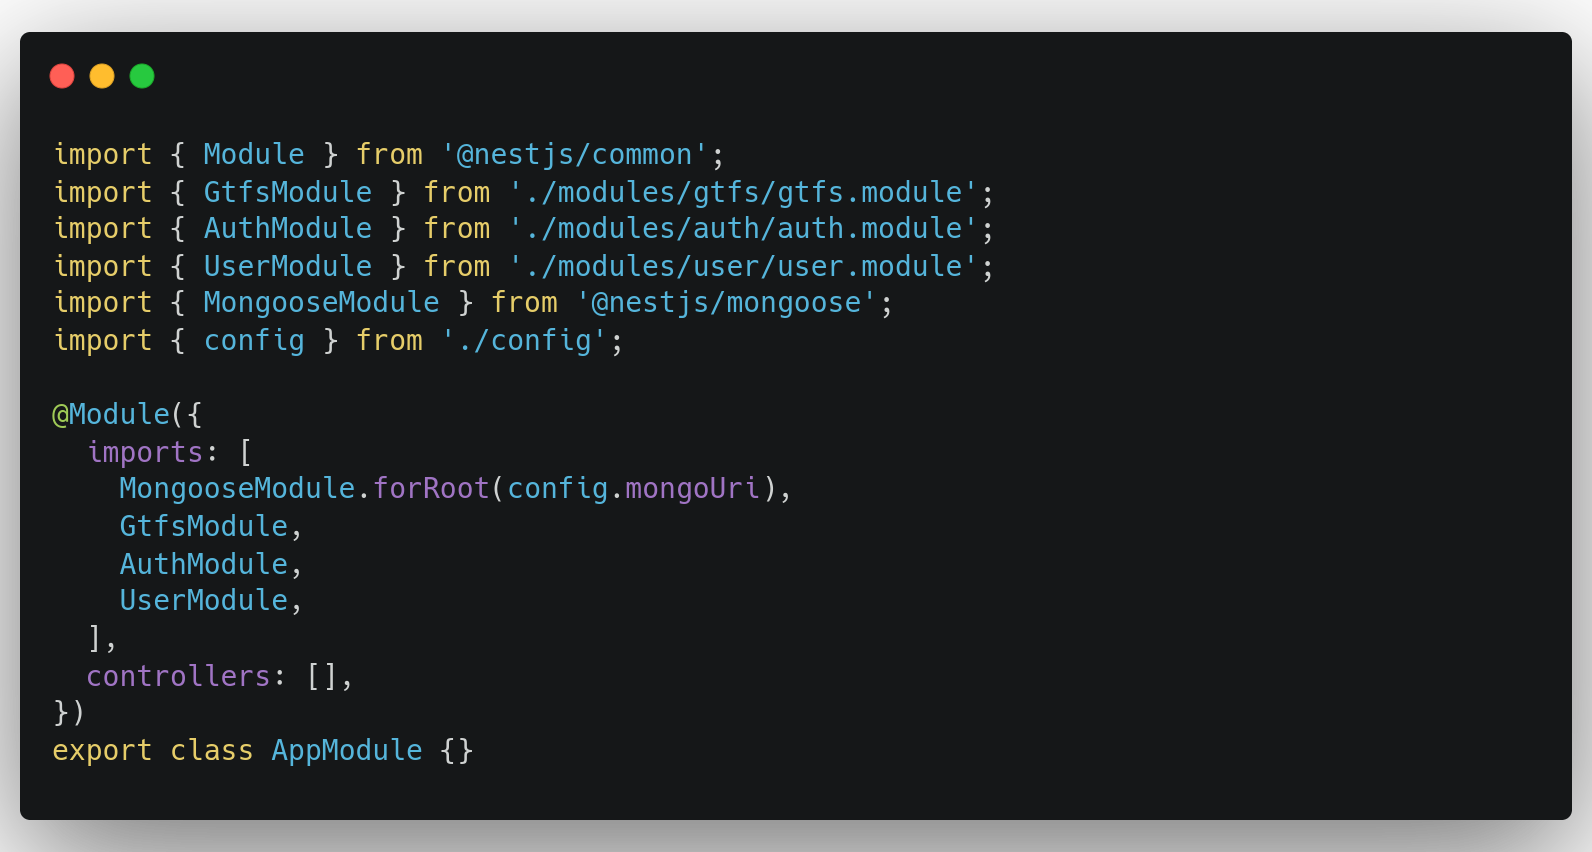
\includegraphics[width=0.9\textwidth]{./figures/code/be_app-module.png}
    \caption{Backend: AppModule.}
    \label{FigBeAppModule}
\end{figure}

\subsection{Configuration}
\label{sec:Configuration}

Backend configuration is stored in a \verb|config.yaml| file at the root of our project. The file is ignored by git, and serves as the location to place all the application secrets and connection instructions, along with configuration that might differ from an environment to the next.

A schema of the configuration file, without actual values, is presented in Figure \ref{FigBeConfig}. We can see configuration related to GTFS (where to download GTFS data from, and what files), along with social authentication secrets, MongoDB database URL, and JWT generation secret.

\begin{figure}[htbp]
    \centering
    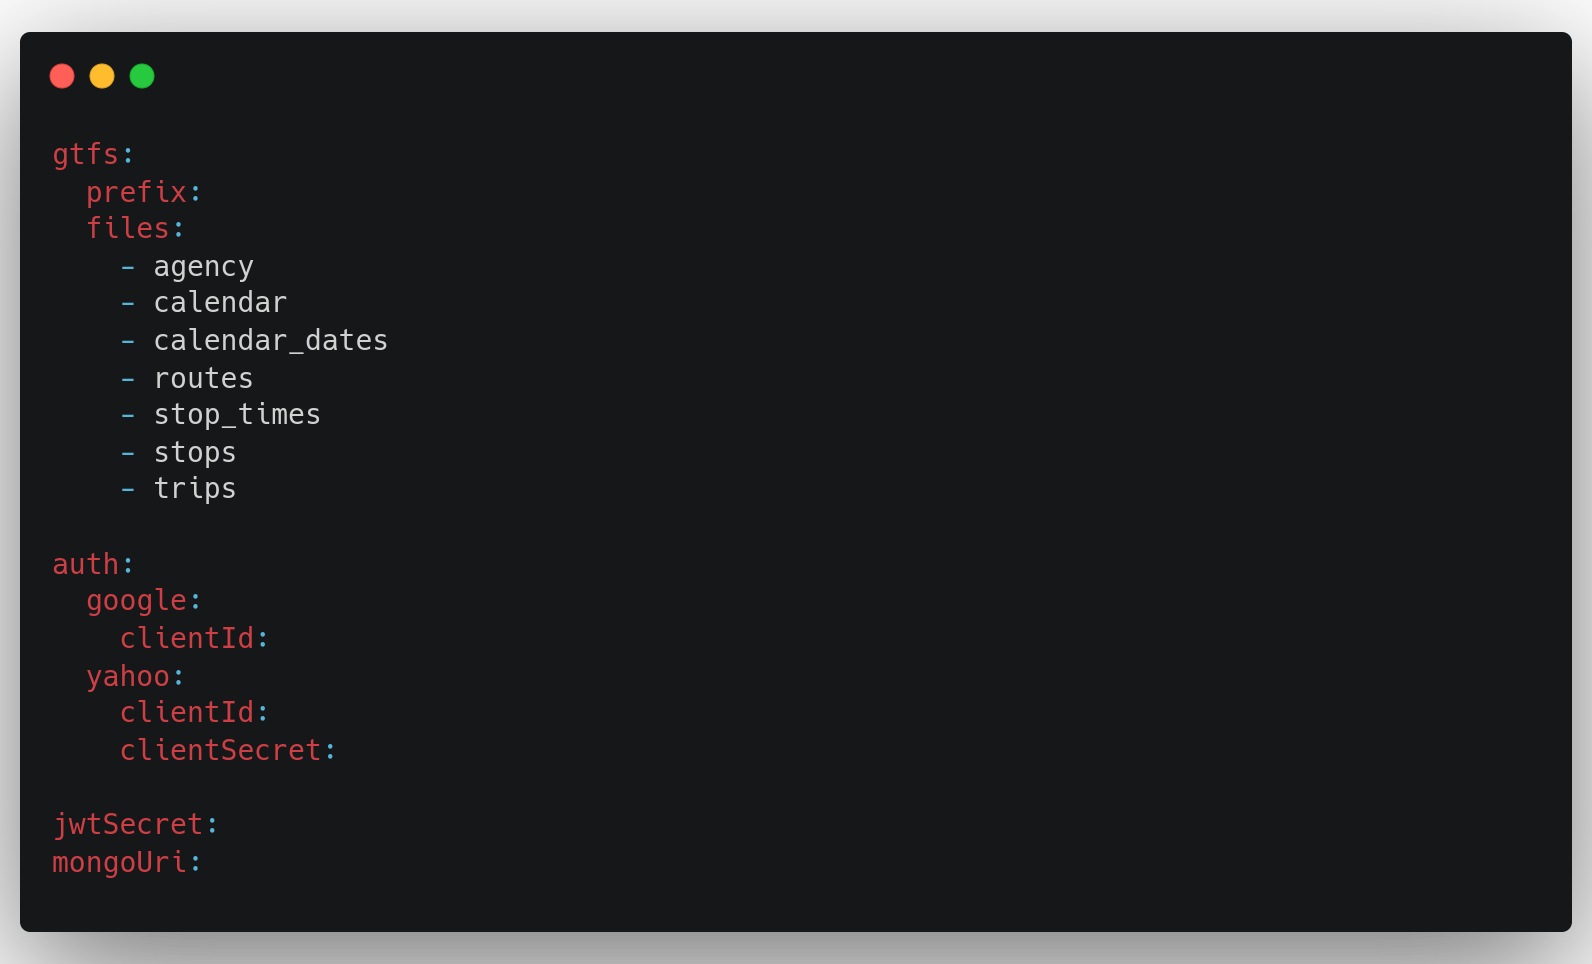
\includegraphics[width=0.9\textwidth]{./figures/code/be_config.png}
    \caption{Backend: config.yaml}
    \label{FigBeConfig}
\end{figure}

The YAML file is then loaded into memory in the \verb|config.ts| TS module, then exported so that it is available for the entire application.

Having the configuration file be loaded by Node is a decision taken in light of simplicity. NestJS offers ways of integrating configuration within its module system, but it requires writing additional code and logic, not only for the providing module, but for modules and services that use the configuration too.

As a safety precaution, the config file is validated against a schema using Joi, which can help identify missing configuration parameters at application startup, rather than have the application crash when it tries to access an inexistent configuration parameter. The Joi schema is presented in Figure \ref{FigBeConfigSchema}.

\begin{figure}[htbp]
    \centering
    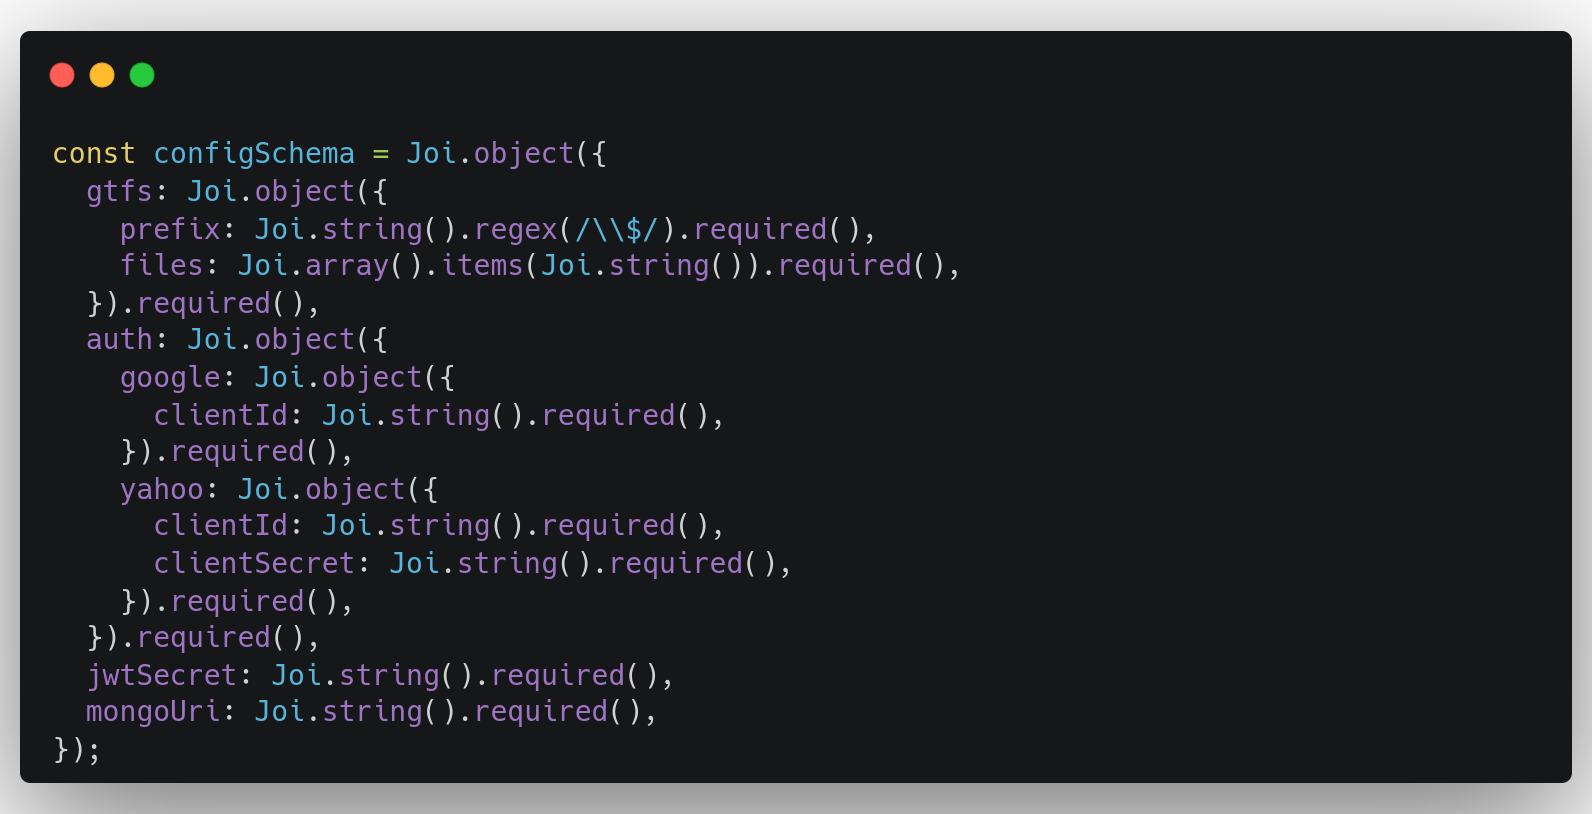
\includegraphics[width=1\textwidth]{./figures/code/be_config-schema.png}
    \caption{Backend: config validation schema.}
    \label{FigBeConfigSchema}
\end{figure}

\subsection{Preparing GTFS data for download}

The GTFS files are available on Vasile Coțovanu's GitHub repository \cite{VasileRubyExporter}, and before serving to our frontend, the files need to be downloaded locally first.

To this end, there exists a script called \verb|process-gtfs.ts|, that when run, creates a Nest application but only loads the GTFS module (Figure \ref{FigBeGTFSBootstrap}). The script then retrieves the \verb|GtfsService| service and uses it to initiate the download of GTFS data from GitHub, which is then placed in the \verb|trip-data| directory. This directory is then referenced in the static assets declaration from the application bootstrapping code (see Section \ref{sec:AppModule}).

\begin{figure}[htbp]
    \centering
    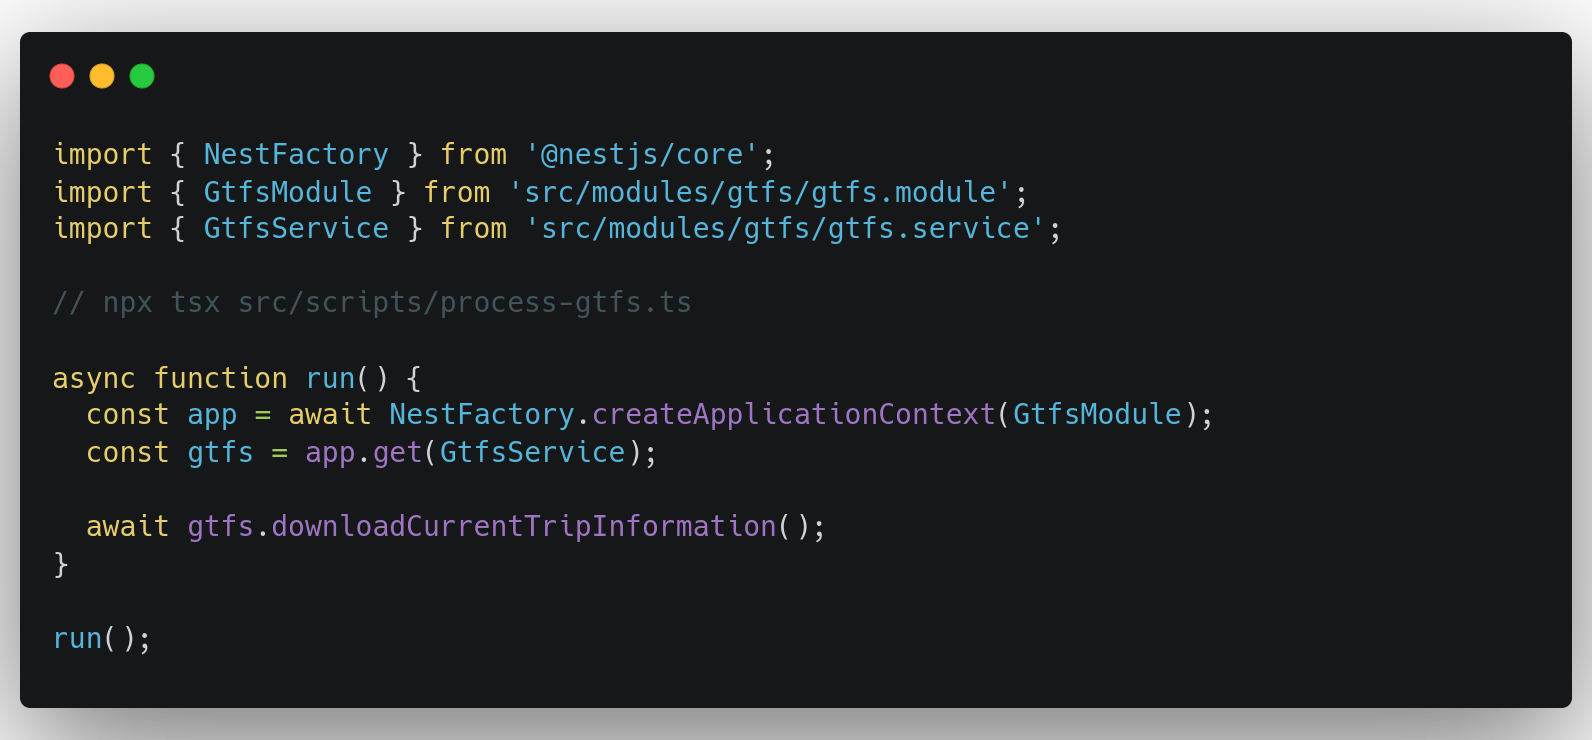
\includegraphics[width=1\textwidth]{./figures/code/be_gtfs-bootstrap.png}
    \caption{Backend: GTFS script bootstrapping code.}
    \label{FigBeGTFSBootstrap}
\end{figure}

\subsection{Auth module}

\begin{figure}[htbp]
    \centering
    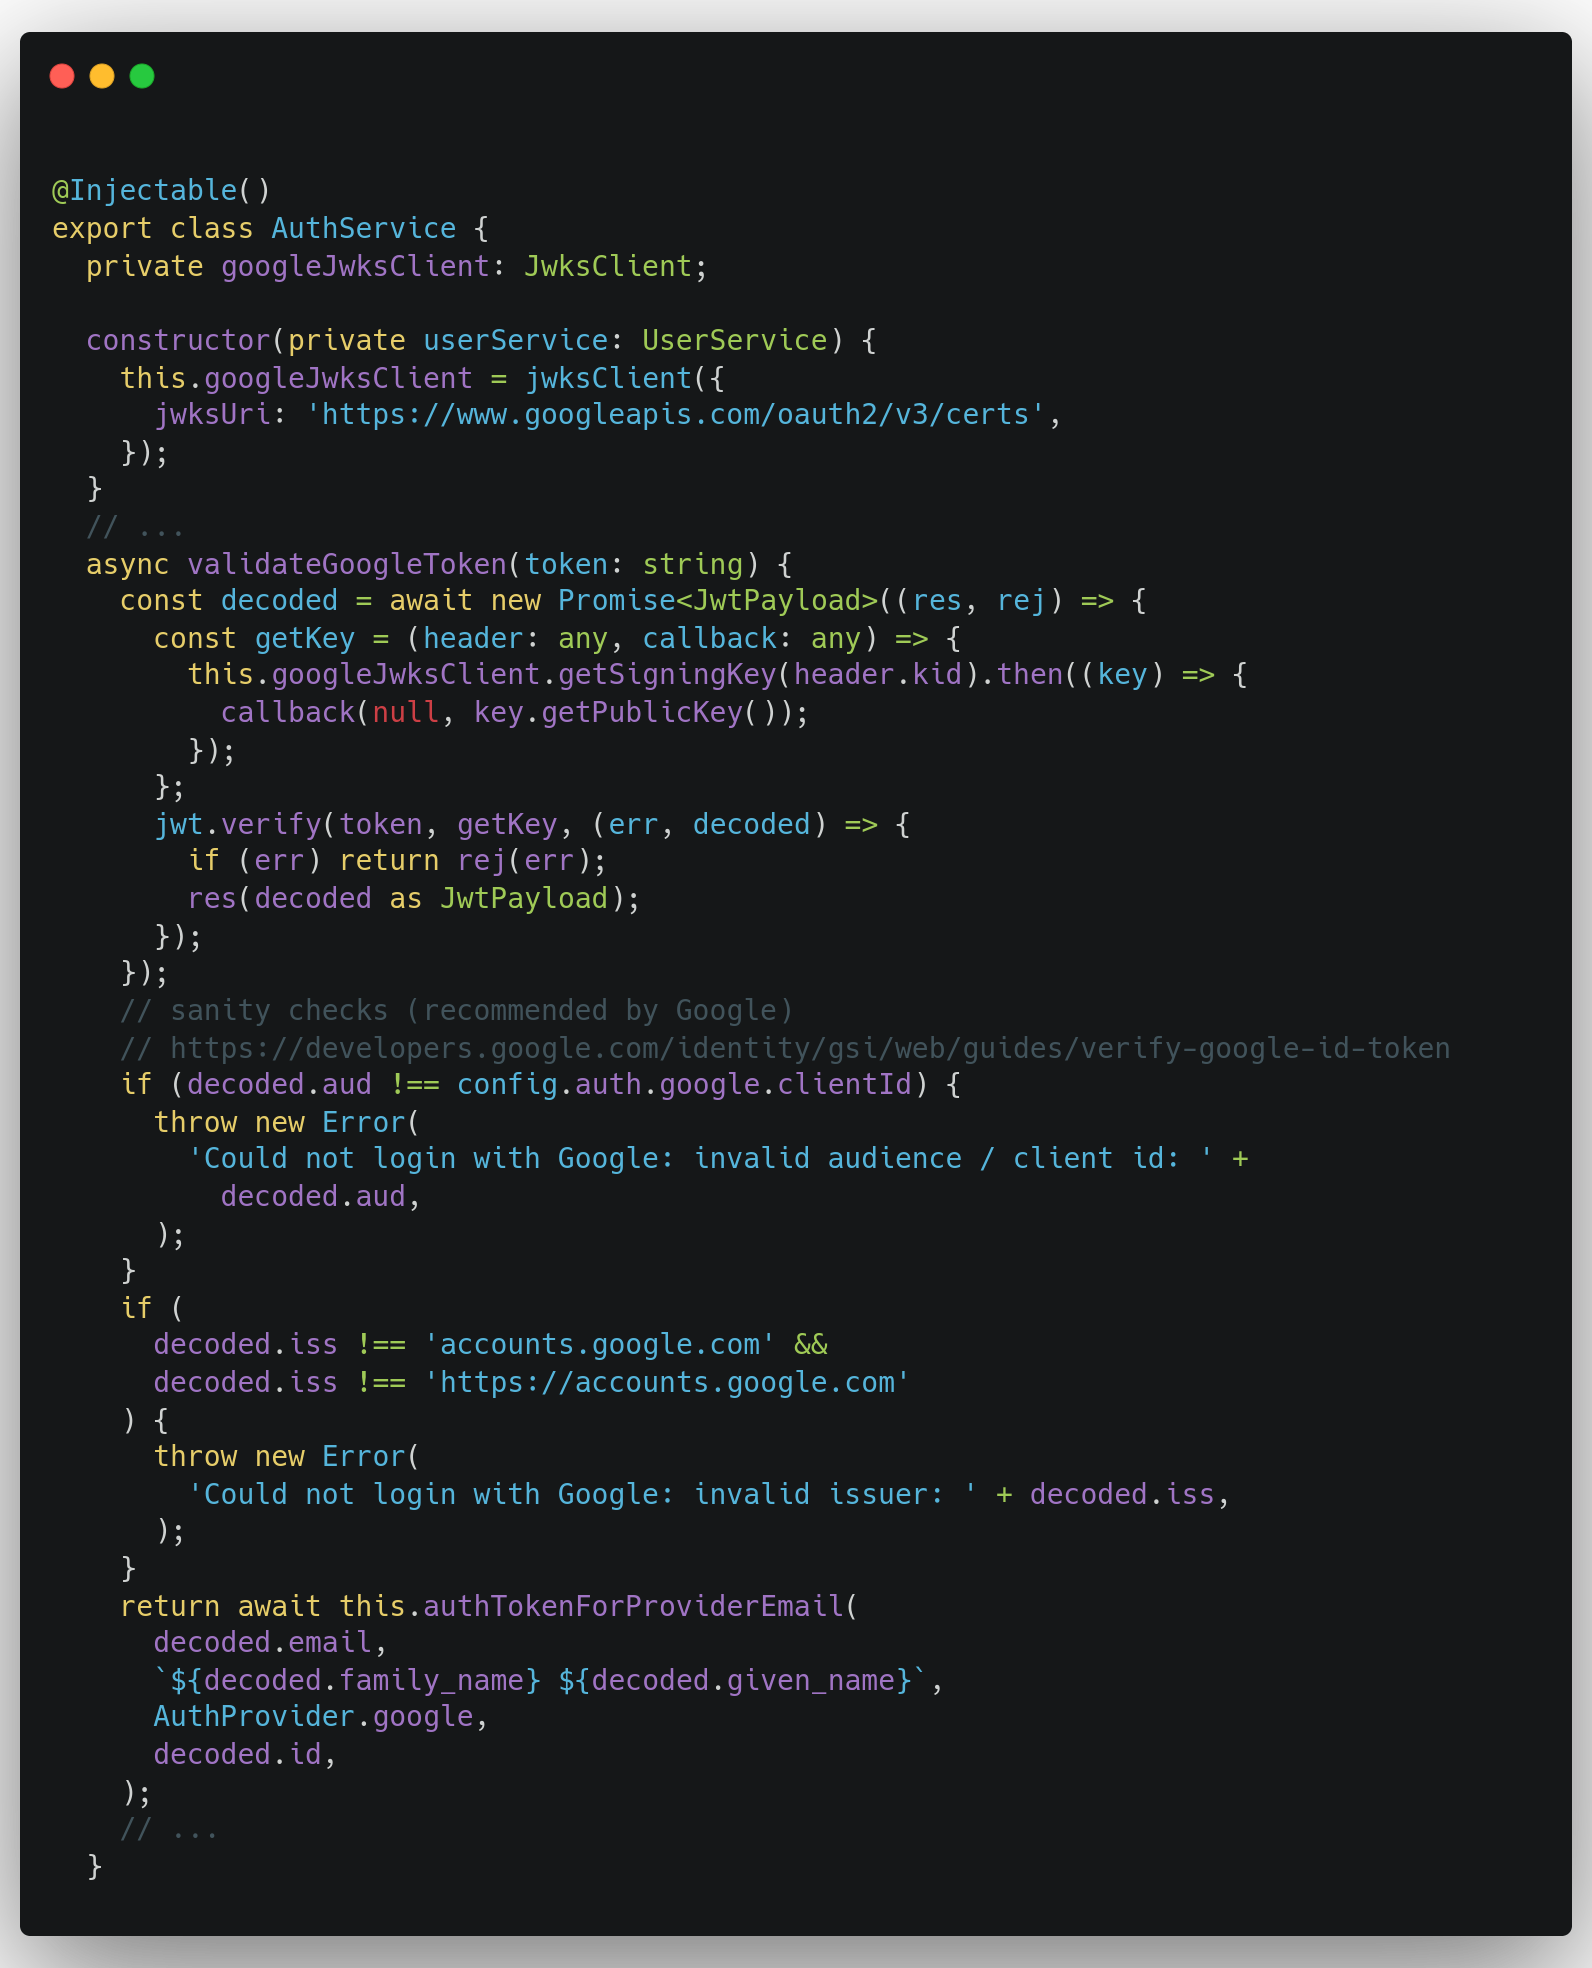
\includegraphics[width=0.9\textwidth]{./figures/code/be_auth-service-google.png}
    \caption{Backend: code that validates Google JWT tokens, for Google sign-in.}
    \label{FigBeAuthServiceGoogle}
\end{figure}

The Auth module has functionality related to user authentication: validating social logins, validating username and passwords, generating JSON Web Tokens (JWTs) and validating those tokens.

Google Sign-in is validated using a token received from the frontend and emitted by Google. The token is a JWT that is encoded using a JSON Web Key (JWK). Google publishes the public keys they use in a JSON Web Key Set (JWKS) format, which can be used to validate JWT tokens emitted from them, and verify their authenticity. Google also recommends performing a set of sanity checks on the JWTs apart from checking their signature, to prevent various attacks, such as emitting valid JWTs for a different application, or from a different Google service. The JWT signature verification library used in the app also makes sure that \verb|iat| and \verb|exp| are enforced (disallowing expired tokens). See Figure \ref{FigBeAuthServiceGoogle} for a code snippet of this step.

Yahoo Sign-in is validated by redirecting the user through a traditional OAuth authorization flow. At the end of the frontend flow, the backend receives a code that will then be sent to Yahoo (using a REST API) for validation, resulting in an \verb|access_token| that grants permission to Yahoo's OAuth APIs. The backend then makes a request to the userinfo endpoint, retrieving the user's email.

Upon validating social credentials, the backend then checks for an user account that already exists in the database (matching using the user's email as received from the social provider), creating one if one doesn't already exist. For this user id, a JWT token is emitted using the application secret (as defined in the configuration, see Section \ref{sec:Configuration}), and returned to the frontend.

The \verb|AuthModule| also provides methods to verify user JWTs, and a Request Guard that can be used to guard API routes that require authentication. Validating JWTs from API requests is done via a library called \verb|passport| and its Nest integration \verb|@nestjs/passport|. Making use of the JWT passport strategy, we can easily configure a strategy that checks JWTs received in the \verb|Authorization| header, via the application's JWT secret. The code is available in Figure \ref{FigBeJwtStrategy}, where it can be noticed how we configure \verb|passport| to validate JWTs, and tell it how to retrieve a user from a valid JWT by making use of the \verb|AuthService|.

\begin{figure}[htbp]
    \centering
    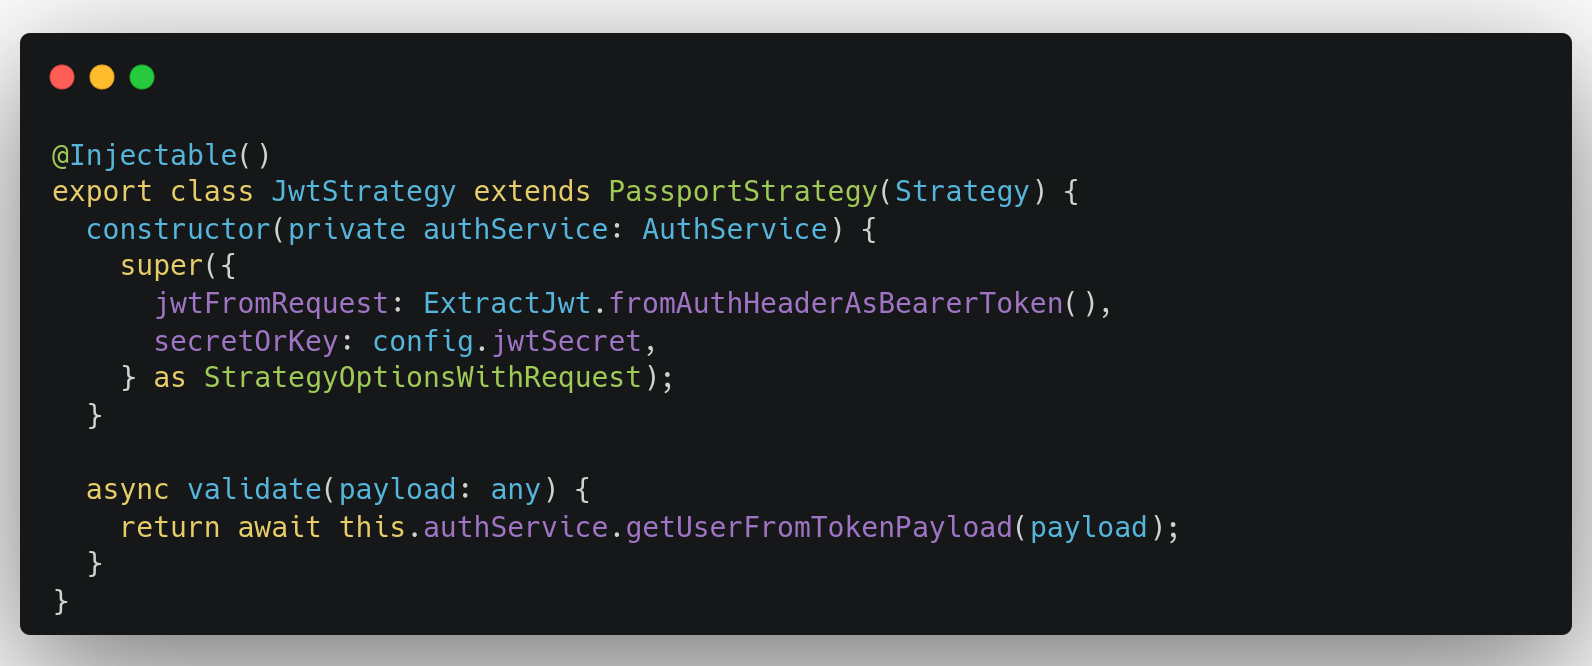
\includegraphics[width=1\textwidth]{./figures/code/be_jwt-strategy.png}
    \caption{Backend: the JWT strategy, as defined using @nestjs/passport.}
    \label{FigBeJwtStrategy}
\end{figure}

A popular method of accessing user data pertaining to a request, in the Express framework, is by attaching a \verb|user| property on the \verb|req| (Request) object. This object is passed around to all handler code in the app, making it an easy way of passing request state around the application. Nest abstracts away this \verb|req| object, and although it provides ways of accessing it, they are discouraged in lieu of a more opinionated approach, that is less prone to type errors. The Nest approach of decoding the user from the request consists of creating a decorator that makes this decoding for us, and places the user object into a parameter of choice in the controller code. The definition of this decorator, along with an example, is shown in Figure \ref{FigBeReqUser}.

\begin{figure}[htbp]
    \centering
    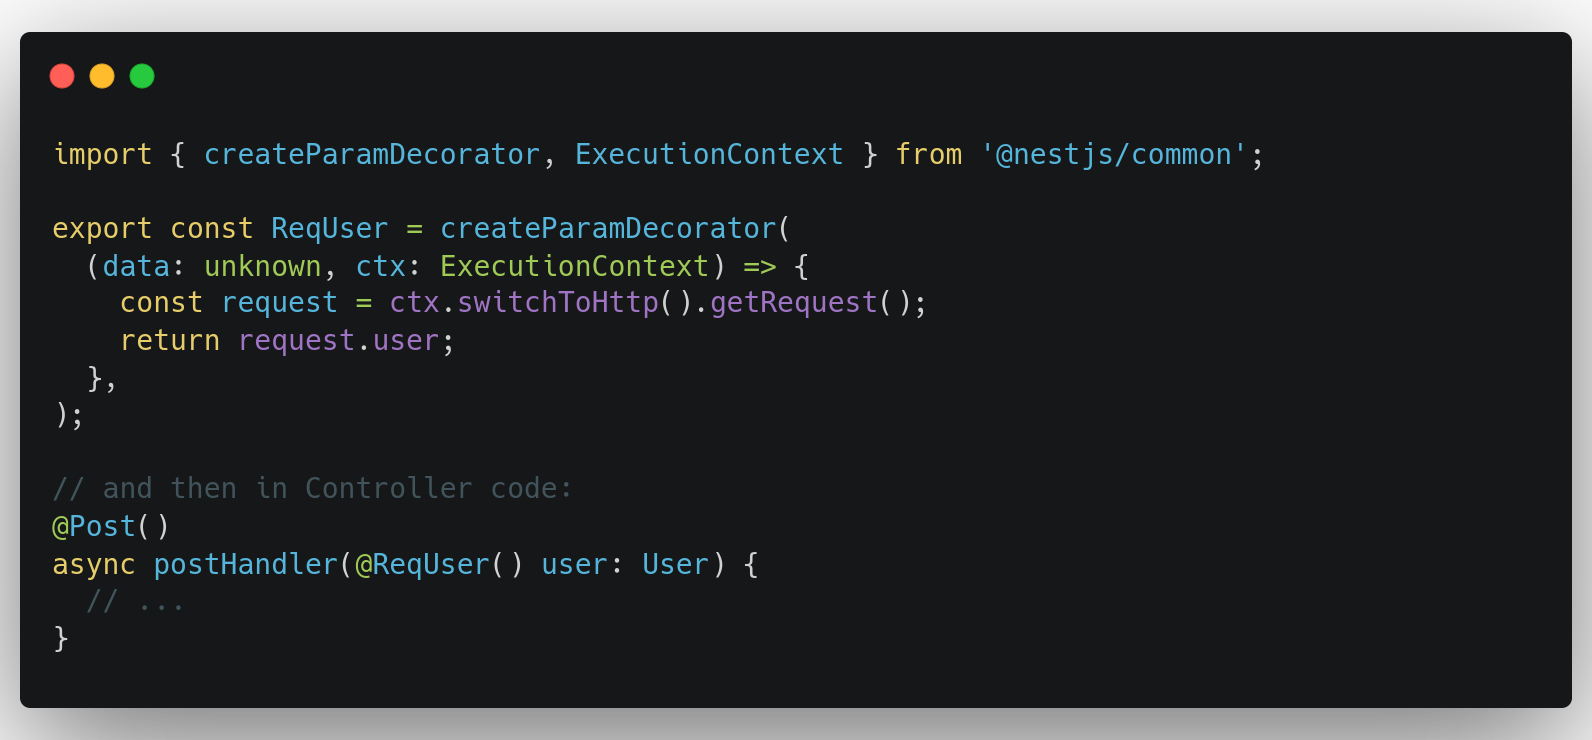
\includegraphics[width=1\textwidth]{./figures/code/be_req-user.png}
    \caption{Backend: the definition of the @ReqUser() decorator, along with an usage example.}
    \label{FigBeReqUser}
\end{figure}

\subsection{DTO validation}

All request validation throughout the app is performed using Data Transfer Objects (DTOs), that are decorated with specific validation criteria.

\begin{figure}[htbp]
    \centering
    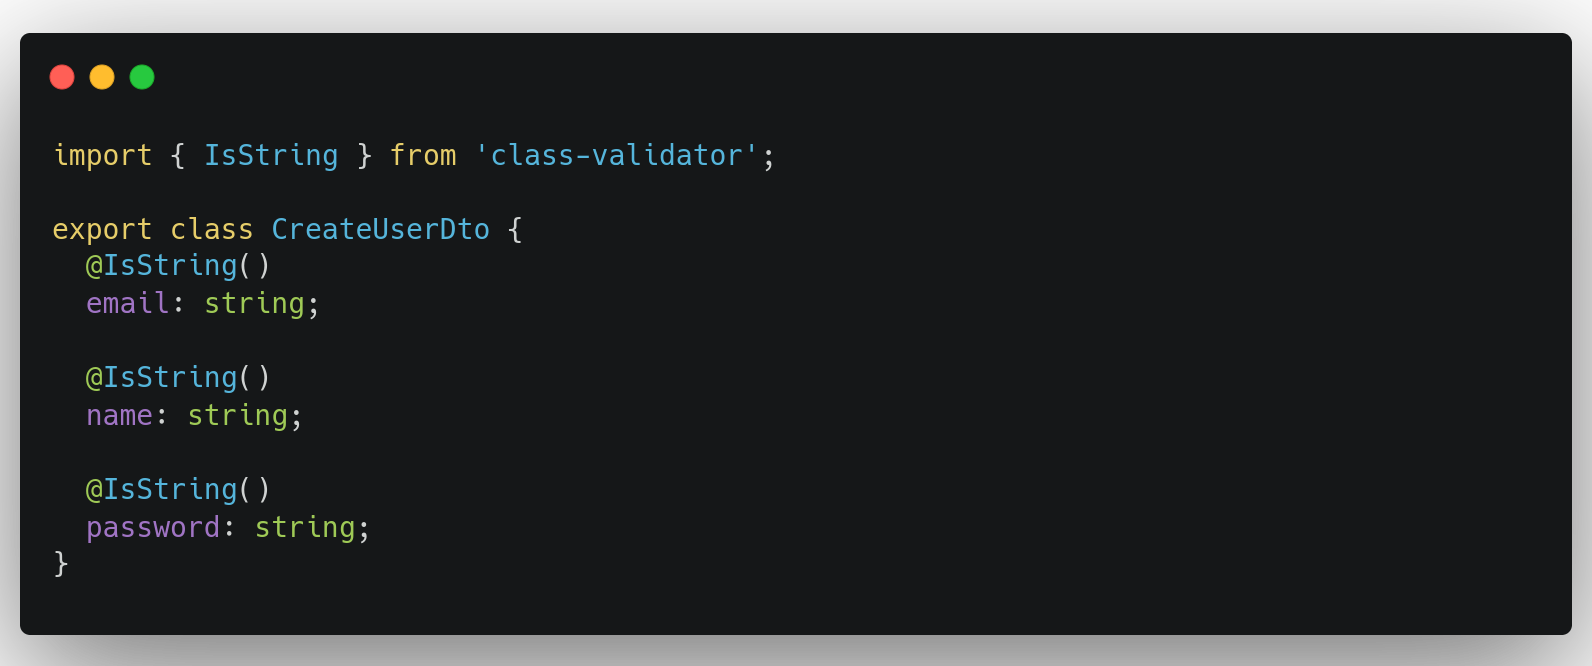
\includegraphics[width=1\textwidth]{./figures/code/be_dto.png}
    \caption{Backend: the definition of a DTO with validation, exemplified on the register request.}
    \label{FigBeDto}
\end{figure}

Figure \ref{FigBeDto} shows how such a validation class looks like. The \verb|ValidationPipe| declared globally (referenced in Section \ref{sec:AppModule}) will use this class decorated with \verb|class-validator| validators to validate the request body of the register endpoint. If a property is found to have a different type to the one specified in the constraint, \verb|class-validator| will throw an error and Nest will return a HTTP 422 status code, with detailed information about how the payload is malformed.

You can notice that the class fields are annotated with TypeScript types (in this case, string). It is important to point out that these types are not enforced at runtime, since they only aid in compile-time type safety. There is nothing to prevent the programmer from adding TS types here that do not match with the decorators, however this mistake is unlikely due to how the decorators are placed right next to the properties.

A special kind of attack can be performed by adding more properties on the request body object that have special significance to other components of the application (for example, MongoDB). By default, the ValidationPipe provided by Nest only checks that those three fields (email, name, password) are valid, but once these checks are complete, the entire request body is deserialized and converted into a JS object, with all its properties. It's then trivial for those properties to be passed to \verb|mongoose| database code, as a byproduct of language features such as the spread syntax (\verb|...obj|), and then have them run arbitrary queries on the database system. To this end, the ValidationPipe offers a configuration parameter \verb|whitelist|, that will remove all extraneous properties that are not explicitly validated in the DTO. If unvalidated properties are desired, the programmer can use the \verb|@Allow()| decorator.

\subsection{User module}
The user module handles users and their trips. The trips are not separated in another module due to how they are stored in the database under the same document, and thus are accessed using the same MongoDB collection (or model, as described by \verb|mongoose|).

\begin{figure}[htbp]
    \centering
    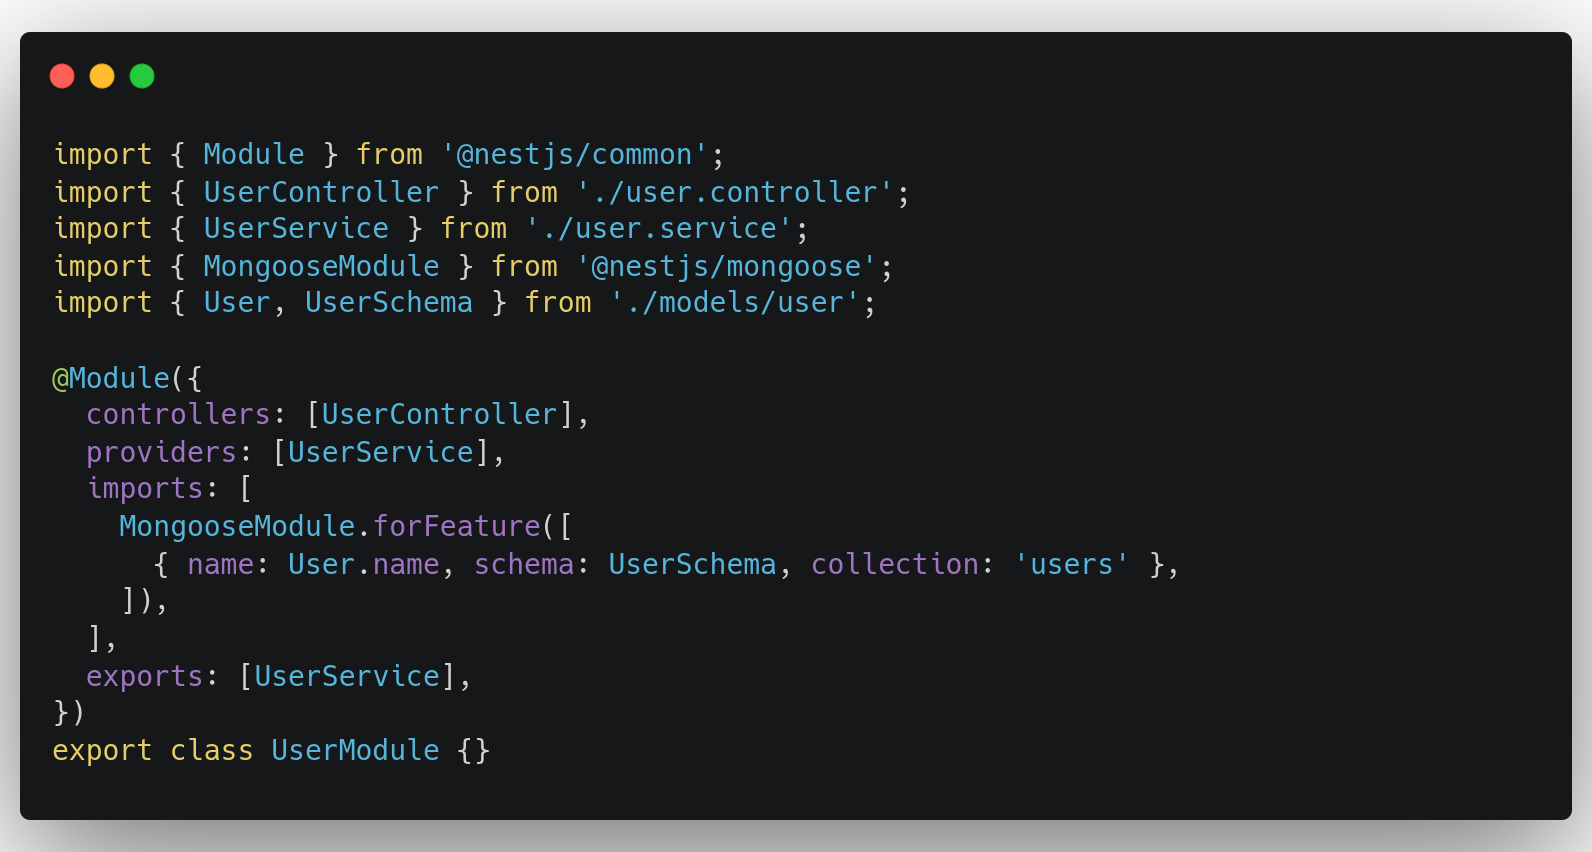
\includegraphics[width=1\textwidth]{./figures/code/be_user-module.png}
    \caption{Backend: the user module.}
    \label{FigBeUserModule}
\end{figure}

Figure \ref{FigBeUserModule} shows the definition of the UserModule. It is interesting to notice the separate parts of the module declaration:
\begin{enumerate}
    \item \textbf{controllers:} represents the list of controllers that this module exposes to the Nest framework. Controllers that are not registered here are not visible to Nest's internal router.
    \item \textbf{providers:} represents the list of providers that this module makes use of. A provider is any class decorated with \verb|@Injectable()|, and all providers are available for dependency injection.
    \item \textbf{imports:} represents a list of modules that this module depends on. Namely, we depend on MongooseModule. However, registering MongooseModule as a root module is not suitable here, since we already imported it as root in AppModule. For this reason, we use \verb|.forFeature()|, which is used to register specific models for use with \verb|mongoose|.
    \item \textbf{exports:} represents a list of all providers that this module exposes to other modules. As a consequence, all modules that import UserModule have access to the UserService. The module that makes use of this service is the AuthModule.
\end{enumerate}

Another interesting analysis we can make is on the User model. The \verb|mongoose| framework makes use of \textit{schemas} to enforce object validation on the documents that get persisted to the database. However, the schemas need to be declared in plain JavaScript, and since they don't integrate well with TypeScript, the mongoose documentation recommends writing the schema twice: once for registering in mongoose, and once for TypeScript type safety.

Nest offers native support for mongoose, and comes with a solution to enable a single class to provide both a mongoose schema, and TypeScript type safety. Visible in Figure \ref{FigBeUserModel}, the solution consists of decorating all class properties using the \verb|@Prop()| decorator, in a manner not unlike the validation performed by the validation library \verb|class-validator|.

All the \verb|@Prop()| arguments are directly passed to mongoose, so as to make the abstraction as minimal as possible. Similarly, all arguments to \verb|@Schema()| are passed to the mongoose Schema constructor.

In this manner, the class is already ready for TypeScript, and only awaits conversion to a mongoose Schema with the Nest \verb|SchemaFactory.createForClass()| method, seen in action in the last line of Figure \ref{FigBeUserModel}.

\begin{figure}[htbp]
    \centering
    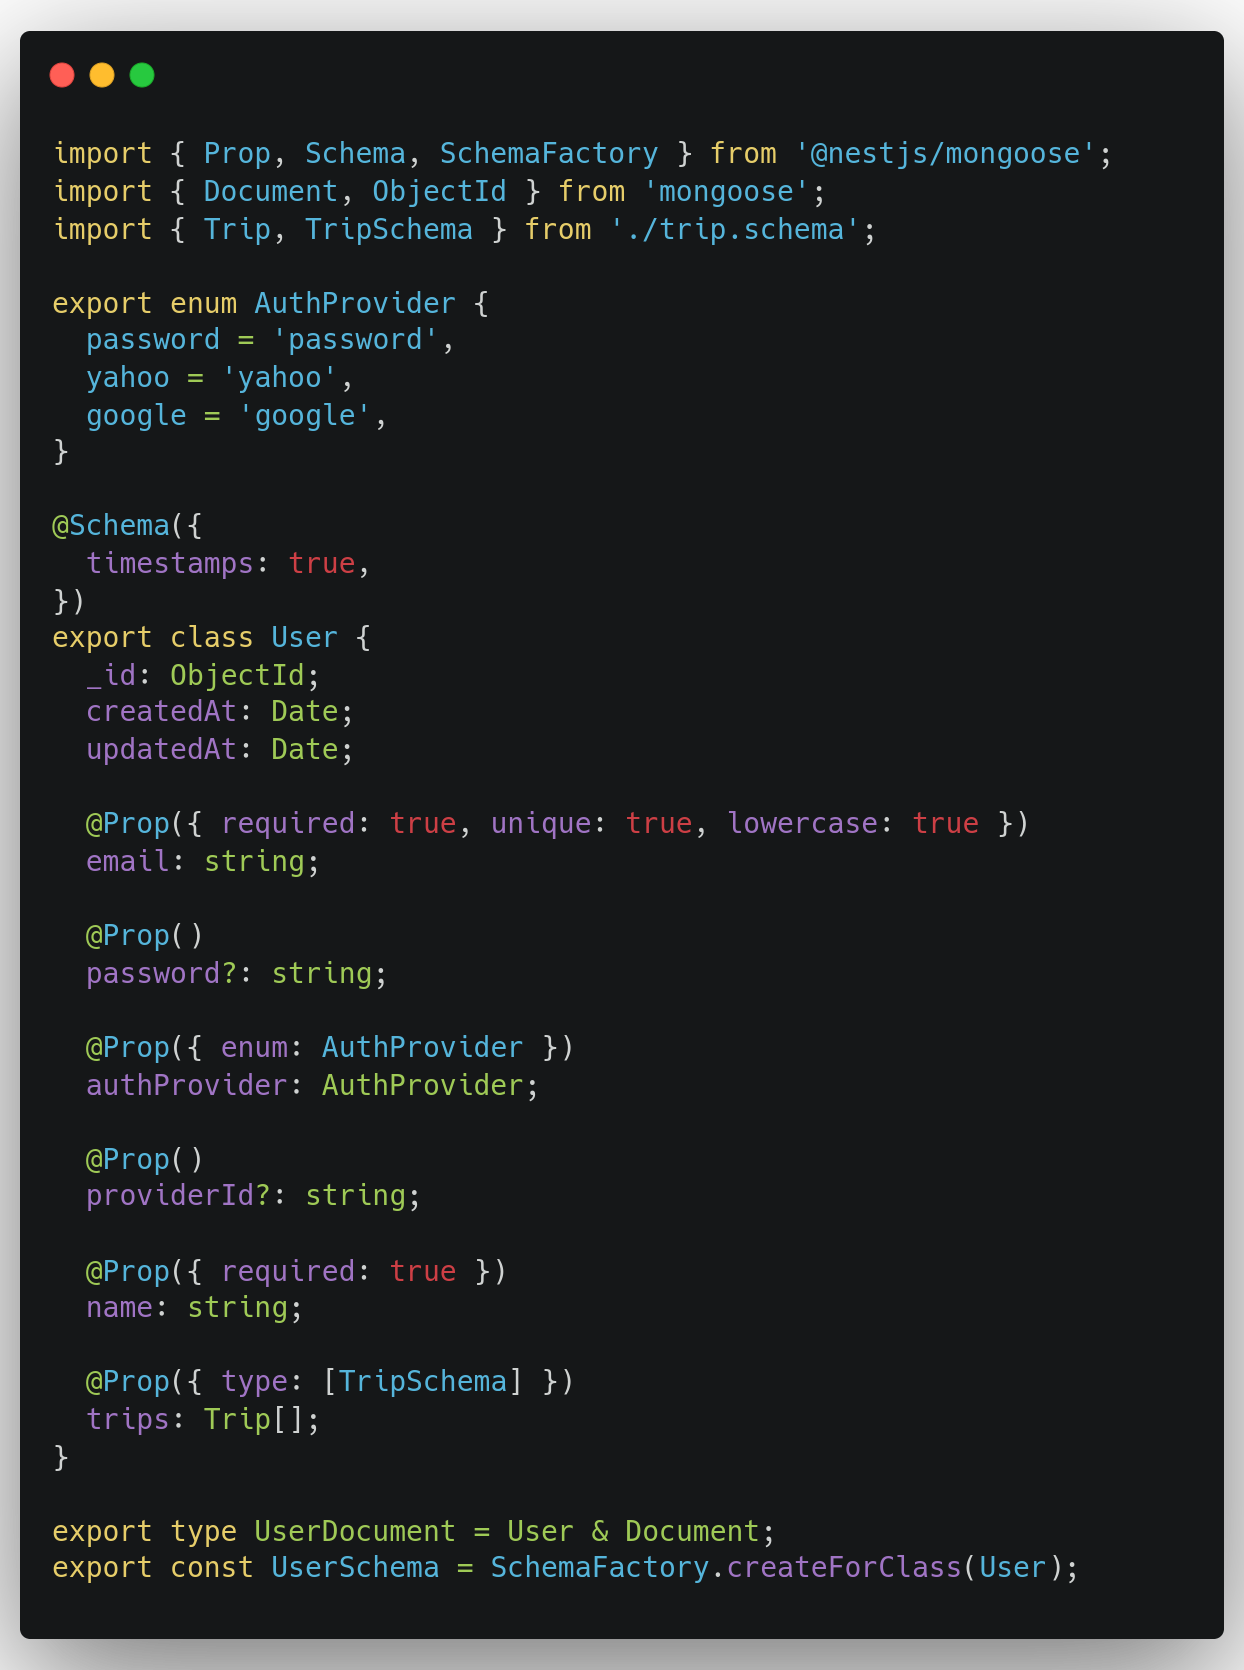
\includegraphics[width=.8\textwidth]{./figures/code/be_user-model.png}
    \caption{Backend: the user model.}
    \label{FigBeUserModel}
\end{figure}

\subsection{Building the project}

Since we employed TypeScript in the project, we are now required to compile the project in order to make it runnable. Albeit running the project directly (the TS files) is possible using tools such as \verb|ts-node| or \verb|tsx|, these tools compile the code on-the-fly, thus making the overall execution slower.

This being said, the compilation does not involve any additional steps apart from the TypeScript compilation.

As such, compiling the project is as easy as running \verb|npm run build| from the root directory of the project. This compiles all TS code and outputs it in the \verb|dist| directory. One can now run \verb|dist/index.js| directly, or use \verb|npm start|, to start the server.

\subsection{Deployment of the backend}
\label{sec:BeDeployment}
Deployment of the backend infrastructure is an interesting case study.

For one, a happy consequence of having the database deployed in the cloud separately is how we don't need to create any special infrastructure for it, since just passing the correct connection URL to the backend application is sufficient for it to successfully connect to it. The database connection is sufficiently fast, even across the Internet (as opposed to on the local computer or even network), as long as the backend and frontend are roughly in the same geographic region (eg. Frankfurt, where both DigitalOcean and Atlas have data centers).

For another, there are cost restrictions imposed on the deployment. I personally own a DigitalOcean droplet (virtual machine in the cloud) that I use for all my projects, so as to have a fixed monthly costs regardless of traffic.

As such, the steps I use to deploy the backend is as follows:
\begin{enumerate}
    \item If first time, clone the repository on the remote machine. Otherwise, just git pull.
    \item Run \verb|npm i| to download or update dependencies.
    \item If first time, make sure the \verb|config.yaml| configuration is suited for production.
    \item Build the project.
    \item If first time, create a \verb|ecosystem.config.js| file, telling PM2 how to run my app (see Figure \ref{FigBeEcosystemConfig}). PM2 is the process manager I use on the VM, that handles app restarts, logs and monitoring.
    \item Run the project using PM2, letting it take over.
\end{enumerate}

\begin{figure}[htbp]
    \centering
    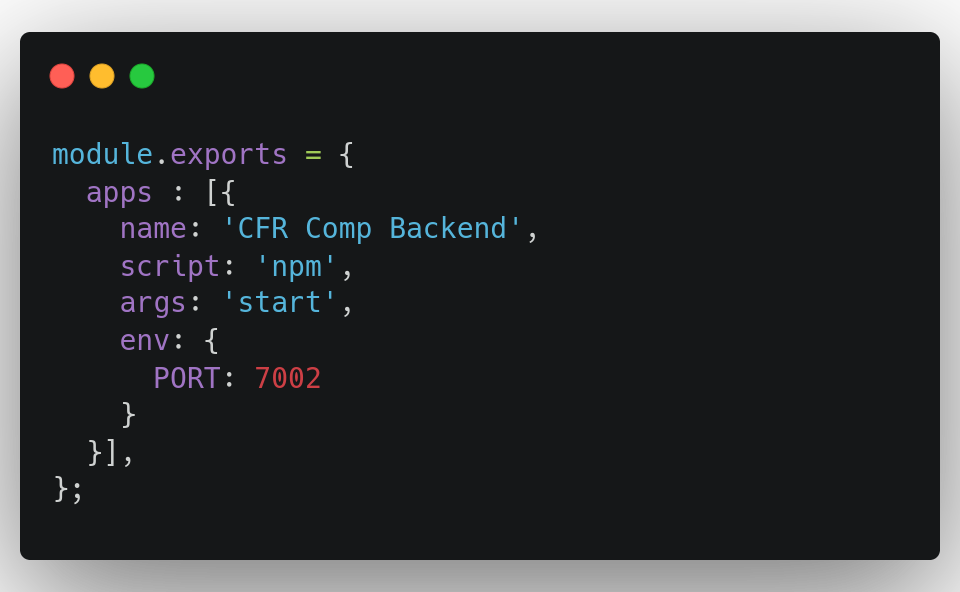
\includegraphics[width=.8\textwidth]{./figures/code/be_ecosystem-config.png}
    \caption{Backend: the ecosystem config, used by PM2 on my personal VM instance.}
    \label{FigBeEcosystemConfig}
\end{figure}

Having a shared virtual machine as a deployment environment proves a challenging task for any continuous integration / continuous development pipelines setup. For this task, I used an application specifically to handle this odd deployment scenario, called Deploy Monkey, available on GitHub \cite{DeployMonkey}. This custom application can link GitHub Actions (by use of webhooks) with my droplet, such that my droplet can automatically run the steps defined above locally, upon notification from GitHub that a push happened.

\section{Frontend application}
Arguably being the most important part of the application, the frontend is written in React with TypeScript and is written to be conformant to the PWA specification, so that it possesses the qualities of a PWA: installable and functional offline.

The bundler used is Vite. The role of a bundler is to take all the different source files and "bundle" them together in a single monolithic file, while also passing the code through all the required compilation steps. In this case, Vite also offers features to help with the development experience, such as hot reloading, and a local web server.

For our purposes, Vite also offers a plugin that helps us convert our application into a Progressive Web Application. We'll explore how this has been done in its own subsection.

\subsection{Functional code}
Modern React does not make use of classes as much as previous versions of it did. In the newer iterations of the library, components are not represented by JS classes anymore, but rather functions, which take the intuitive name of functional components.

\begin{equation}
    \label{eq:StateView}
    f(state) = view
\end{equation}

While classes were the de-facto standard way of writing React code for a long time, they lead to a lot of boilerplate code that could easily have been avoided using functional components. These components were possible back then too, but they were extremely limited in functionality and capability, until React unveiled \textit{hooks}, which changed the functional component scene.

Functional components are extremely intuitive due to how they closely map to the identity presented in Equation \ref{eq:StateView}. In the same manner that a view is a function of the state, a React functional component is a function that returns JSX code based on its parameters (or, how React calls them, \textit{props}).

While, in an ideal world, the above identity would be sufficient to write applications, it must be recognized that React components must do extra things other than calculate views based on their props. As such, React exposes a variety of hooks, that can be called from functional components. These hooks are normal JavaScript functions that "hook" into the React framework and let your functional component keep its own state, make it react to changes in props (or state), or let it perform side-effects as a result of state changes (eg. API calls).

These hooks, while normal JS functions as far as the language is concerned, do carry additional responsibility, due to the way they work with the framework. These restrictions are synthesized into the Rules of Hooks, and they look as follows:

\begin{enumerate}
    \item \textbf{All hook names must begin with 'use'.} For example, \verb|useState|, \verb|useEffect|.
    \item \textbf{Hooks must always be called in the same order.} React keeps track internally of this order to be able to return the correct values for consecutive render calls.
    \item \textbf{Hooks must never be called conditionally.} React will exhibit undefined behavior when a function render performs different hook calls than its previous render. There are situations where conditional hooks are desired, but they must be implemented differently, to avoid breaking the Rules of Hooks.
\end{enumerate}

Our application exclusively makes use of functional components, using hooks. Several custom hooks are also defined, that enable specific application functionality such as authentication, localization, or trip data updates.

\subsection{Pages}
Pages are laid out in a folder structure that closely reflects their URL, under the \verb|pages| directory. The website root layout is defined in the \verb|App.tsx| module, and it takes care of rendering the top navigation bar, along with rendering the child page using React Router.

Rendering of different pages was accomplished using React Router. Using this library is as easy as defining the hierarchy of pages, and using a couple of custom anchor link components instead of the HTML native \verb|<a>| tag.

Figure \ref{FigFeRouter} presents the routing definition, and it is easy to see how the App component is defined as the root page, with the children being the HomePage and TrackPage components.

An odd presence here is the YahooAuthPage, but it is justified by how the Yahoo OAuth authorization flow requires a callback URL to redirect to after the user grants permissions. This page will take the authorization code from the URL and pass it to the API.

\begin{figure}[htbp]
    \centering
    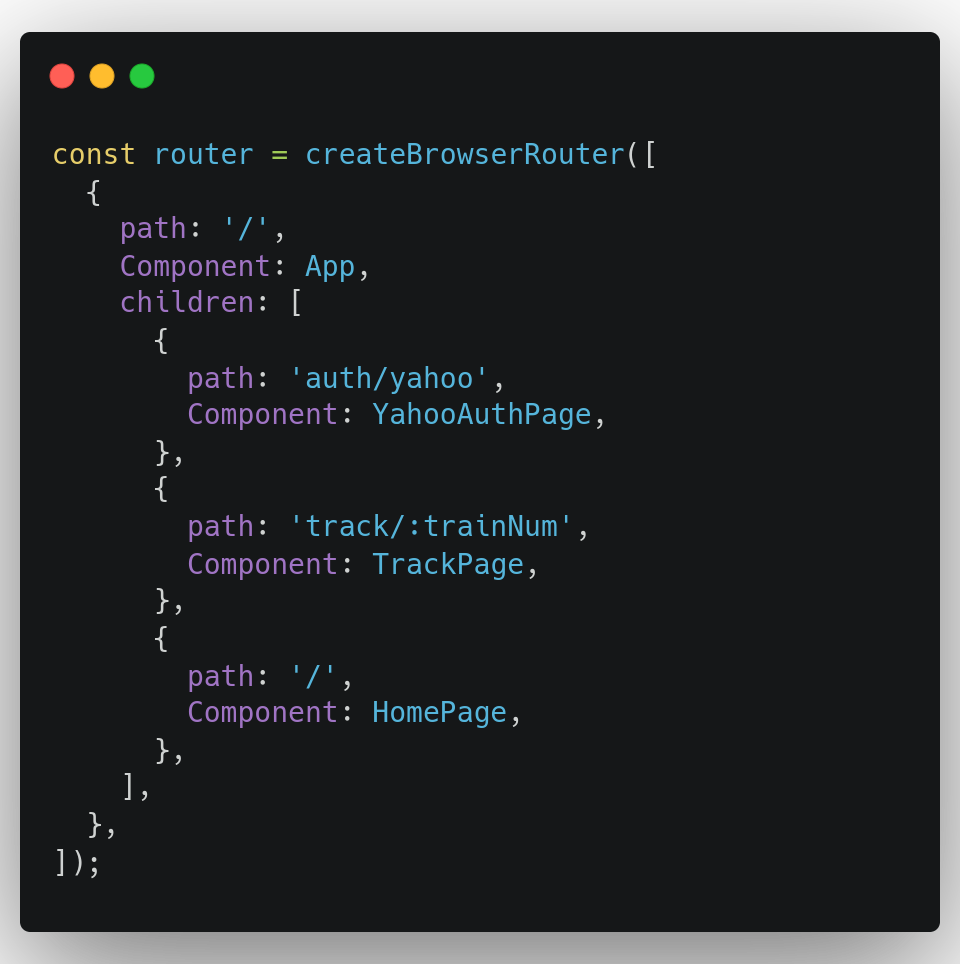
\includegraphics[width=.6\textwidth]{./figures/code/fe_router.png}
    \caption{Frontend: the application router.}
    \label{FigFeRouter}
\end{figure}

\subsection{Contexts}
While state can be declared in parent components and passed down to every component that needs it, state that is required in a lot of components across the component tree might require to be passed through components that make no use of it, and will generally lead to a phenomenon called \textit{prop drilling}.

While there exist a number of libraries that offer global state, such as \verb|zustand|, React does offer its own solution to this issue, in the form of \textit{contexts}.

A context takes the form of a plain JS object that can be declared at the top of the component hierarchy using a Provider, and that can be later accessed at any point in the tree using the \verb|useContext| hook.

Figure \ref{FigFeContexts} shows the React \verb|createRoot| call, and features all the context provi\-ders that the application makes use of. These provider components are plain functional components that keep their own relevant state, and that wrap their children in the React Context Provider component, which makes their state globally available.

\begin{figure}[htbp]
    \centering
    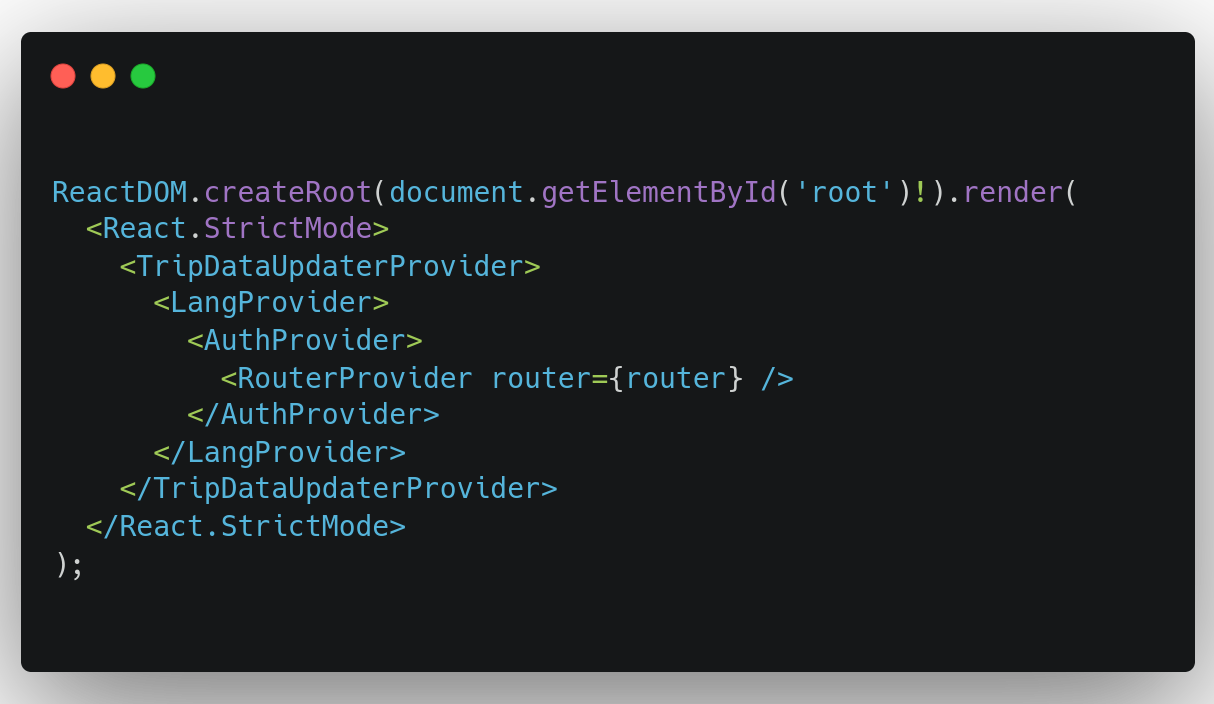
\includegraphics[width=.8\textwidth]{./figures/code/fe_contexts.png}
    \caption{Frontend: the createRoot call, featuring all the context providers.}
    \label{FigFeContexts}
\end{figure}

\subsection{IndexedDB wrapper: Dexie}
IndexedDB is a browser native capability, but its API is deemed to be somewhat hard to use. It technically is async, but has a lot of weird restrictions in place that prevent it to be used in a truly async fashion.

As a consequence, I have decided to use Dexie.js as a wrapper around the IndexedDB functionality. Dexie is able to handle different use cases, such as database migrations, minimal schema validation, TypeScript integration, and indexes. One bonus feature that helped during development was its integration with React, being able to hook into React state and run queries reactively.

\begin{figure}[htbp]
    \centering
    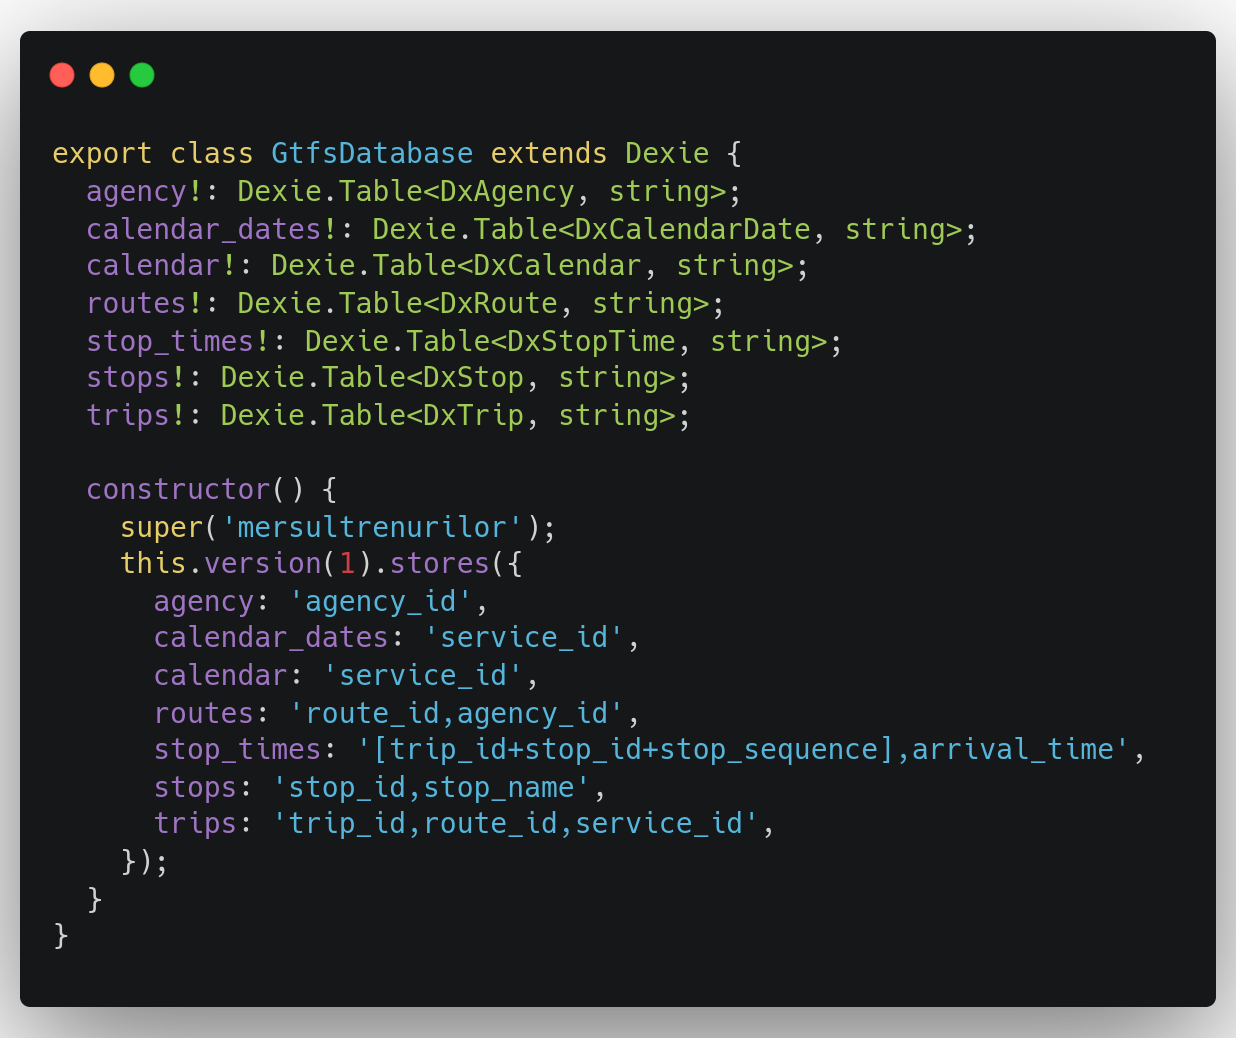
\includegraphics[width=.8\textwidth]{./figures/code/fe_dexie-gtfs.png}
    \caption{Frontend: setting up the Dexie GTFS database.}
    \label{FigFeDexieGTFS}
\end{figure}

Figure \ref{FigFeDexieGTFS} shows the declaration of the GTFS database class. It directly extends the Dexie class, meaning that it exposes all Dexie functionality, but in addition, on instantiation, it automatically sets up the database for use with our GTFS data.

The first few lines represent purely TypeScript support. To make TS aware of our tables, we need to explicitly tell it that they exist, and we provide a interface that it can then do type-checking against. The interfaces are all prefixed with \verb|Dx| to differentiate them from API entities.

The constructor then calls the parent constructor with the name of the database (\verb|mersultrenurilor|), which is followed by the schema definition. While Indexed\-DB does not make use of structured tables and schemas in the same manner as MySQL would, it does need to create tables and set up search indexes on them. Dexie will create all the tables listed in the \verb|stores| call, and set up all the comma-separated indexes. The first value of every enumeration will be considered a \textit{key}, which is functionally equivalent to a primary key in relational databases.

You can notice a special syntax in the \verb|stop_times| definition. That syntax has the effect of creating a \textit{composite primary key}, since all stop times are determined by their trip, stop, and stop sequence.

It is important to notice how the index lists are not covering the entire object they store. IndexedDB can store \textit{any} plain JS object, and it does not place restrictions on what shape those objects can have. As such, the indexes only take the role of a speed enhancement, and not of a restriction.

\subsection{Loading offline GTFS data}
Downloading the GTFS data is always done on page load. The application does a check online to see when the GTFS data has been last updated, and compares it to the last download date it has locally (in the IDB store). If there is newer data on the server, it downloads into memory the entire contents of the GTFS data files, and then uploads them into the IndexedDB database.

This process can take a while, and for this reason the application displays a banner to inform the user that travel data is inaccurate for the duration of the download process.

The banner is visible in Figure \ref{FigFeUpdateBanner}.

\begin{figure}[htbp]
    \centering
    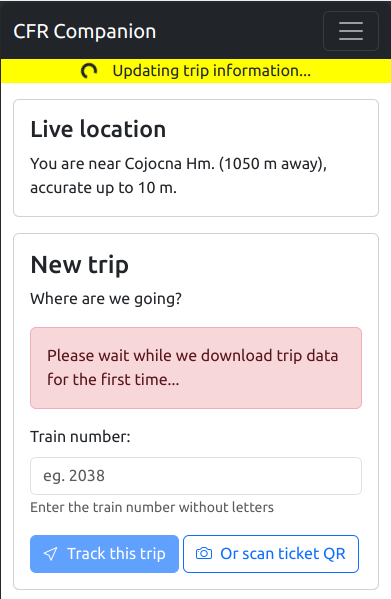
\includegraphics[width=.6\textwidth]{./figures/code/fe_update-banner.png}
    \caption{Frontend: the banner for when travel data is being updated.}
    \label{FigFeUpdateBanner}
\end{figure}

Various components need to know the state of the data update (whether it is checking for updates, what download decision has been taken, whether it is currently downloading or not, or whether it is the first time or not), so the state is provided to the entire application via a context. An usage example is visible in Figure \ref{FigFeUpdateBanner}, where the \textit{New trip} component displays a warning.

\subsection{Internationalization}
Internationalization was a fairly easy process, and it was done without using any third-party libraries. The way it works is by using a React context to provide the currently selected language, and then have the language provider \verb|LangProvider| provide a translation function.

The translation function takes in a translation key (eg. \verb|newTrip.trackBtn|), tries to find the translated string in the locale object (by parsing the object tree from the dot notation), and returns the translated string for use in JSX.

The translation function is reactively updated on changes to the selected language, such that it always returns values from the proper locale, and triggers UI updates across the component tree upon language selection.

In addition, the translation function takes any number of additional string parameters that get interpolated in the output string via numerical markers placed in the locale string (eg. \verb|$1|).

Another feature of the LangProvider is how it saves to the IDB store the currently selected language, and then, on application startup, it looks in IDB and loads up the last selected language. If it finds no selected language, it defaults to the user's navigator language, or English if that language is not recognized.

\begin{figure}[htbp]
    \centering
    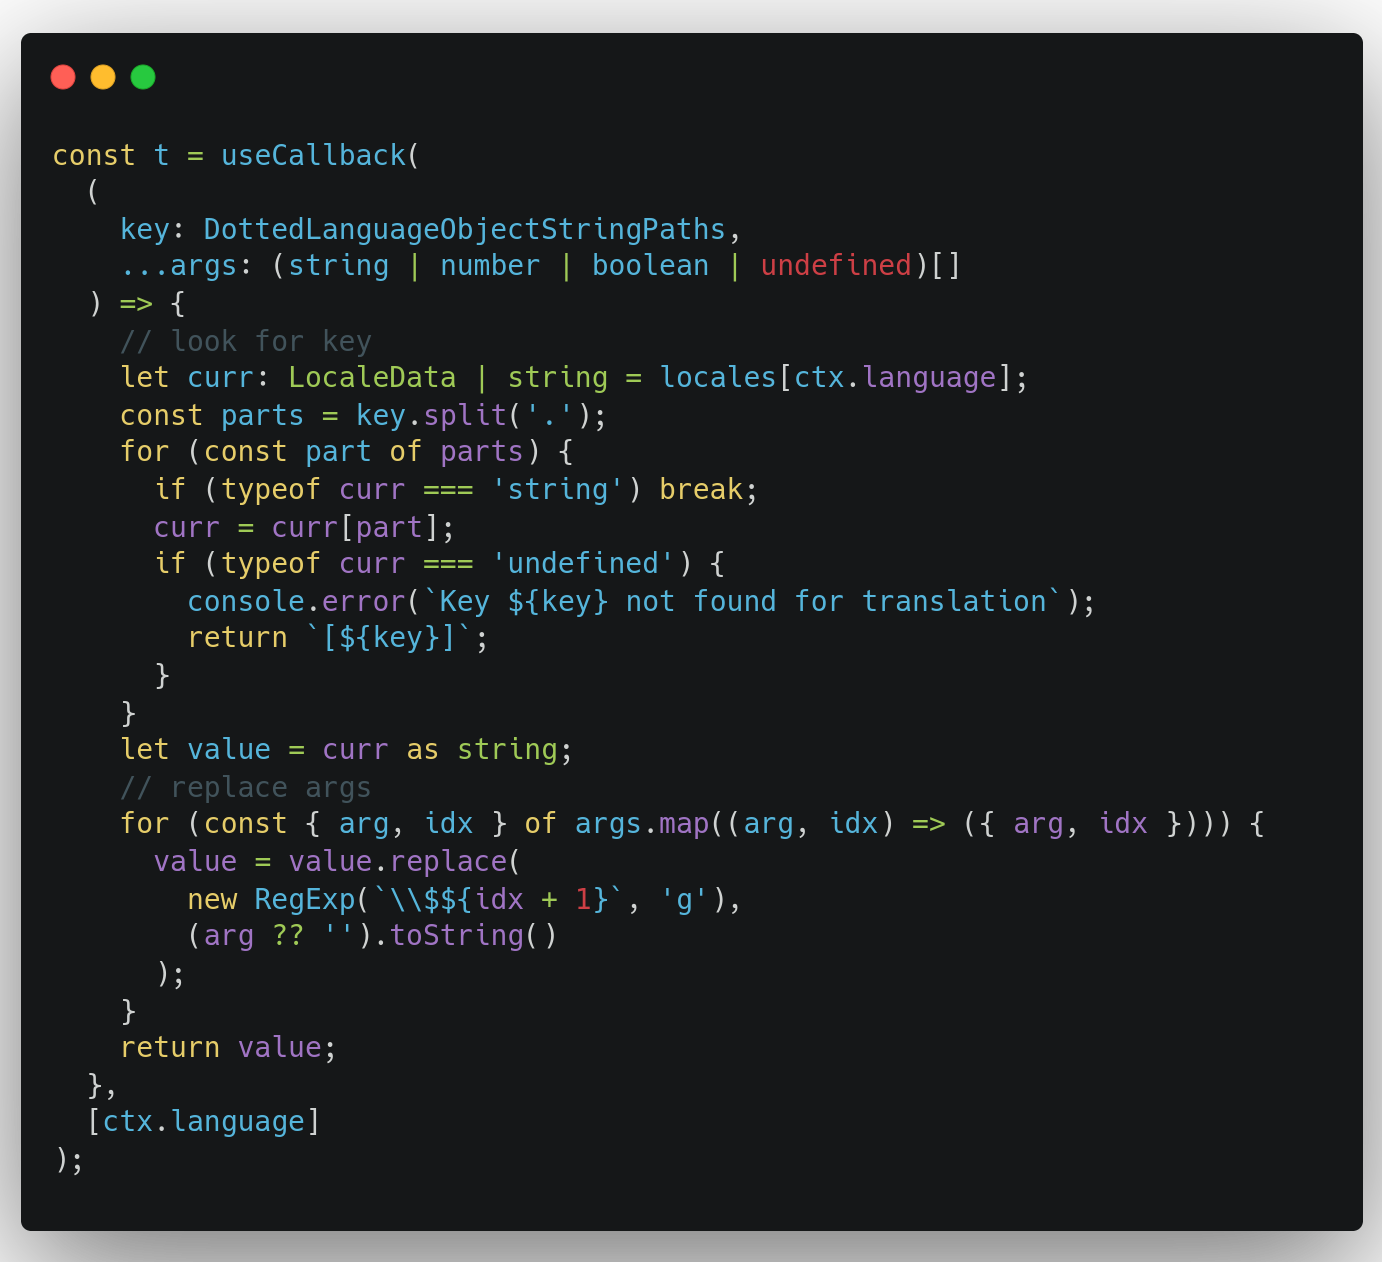
\includegraphics[width=.7\textwidth]{./figures/code/fe_translate-fn.png}
    \caption{Frontend: showcase of the translation function.}
    \label{FigFeTranslateFn}
\end{figure}

Figure \ref{FigFeTranslateFn} presents the translation function employed by the application. First\-ly, the function definition is wrapped in a React \verb|useCallback| hook, that will return the same function reference on subsequent renders (to help reactive code not react if nothing changed), but will return a different function reference when the \verb|ctx.language| value changes.

The function can be seen parsing the locale object of the currently selected locale (using the value of \verb|ctx.language|) and retrieving the proper locale string. If no such string is found, a default value of \verb|"[key]"| is provided.

Afterwards, the function will look in the arguments it has received and start replacing all occurrences of interpolation parameters with the proper values.

Once this process is done, the localized string is ready, and is returned.

An usage example of this translation function can be seen in the next subsection, in Figure \ref{FigFeLiveJsx}.

\subsection{Live location: nearest station}
On the home page, there exists a component whose role is to tell the user (using your live location) what station they are closest to, what distance separates them from it, and to what precision the app knows their location.

This is accomplished by running a query against the IDB GTFS store to retrieve all stations in Romania (totaling around 1700 stations) with their coordinates, calculating the distance to every one of those stations, then using the station with the lowest distance. This query is then repeated whenever a live location update occurs.

React's reactive way of writing application really shined in this context, since no special code had to be written to handle changes, because React simply took care of everything.

\begin{figure}[htbp]
    \centering
    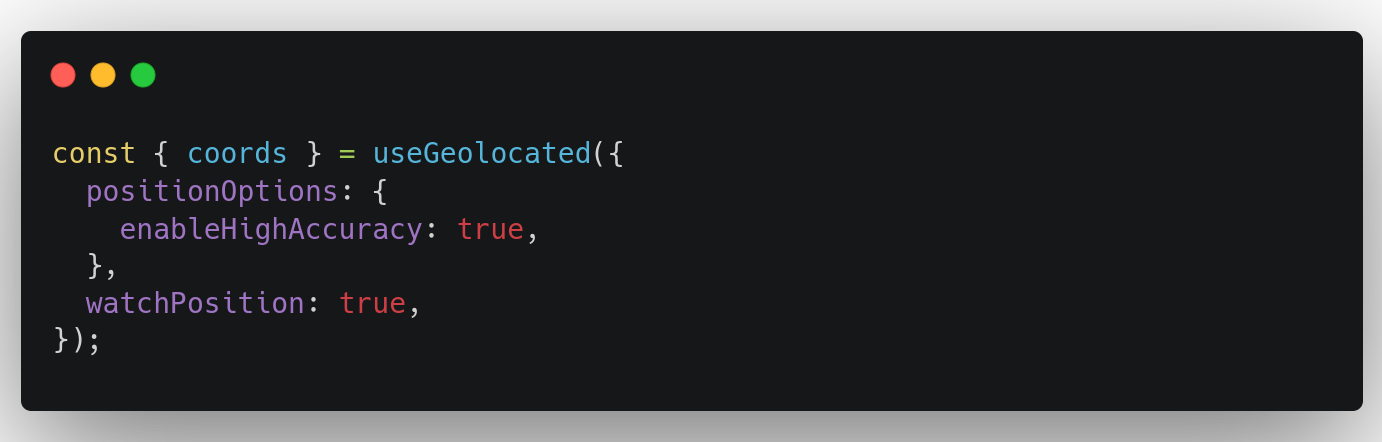
\includegraphics[width=.9\textwidth]{./figures/code/fe_live_coords.png}
    \caption{Frontend: usage of the useGeolocated hook to retrieve coordinates in real time.}
    \label{FigFeLiveCoords}
\end{figure}

Figure \ref{FigFeLiveCoords} shows how the \verb|react-geolocated|'s \verb|useGeolocated| hook was used to hook into the live location of the user. This hook will ask permission from the user to begin location tracking, then return the user's current location, while triggering re-renders every time this location updates.

\begin{figure}[htbp]
    \centering
    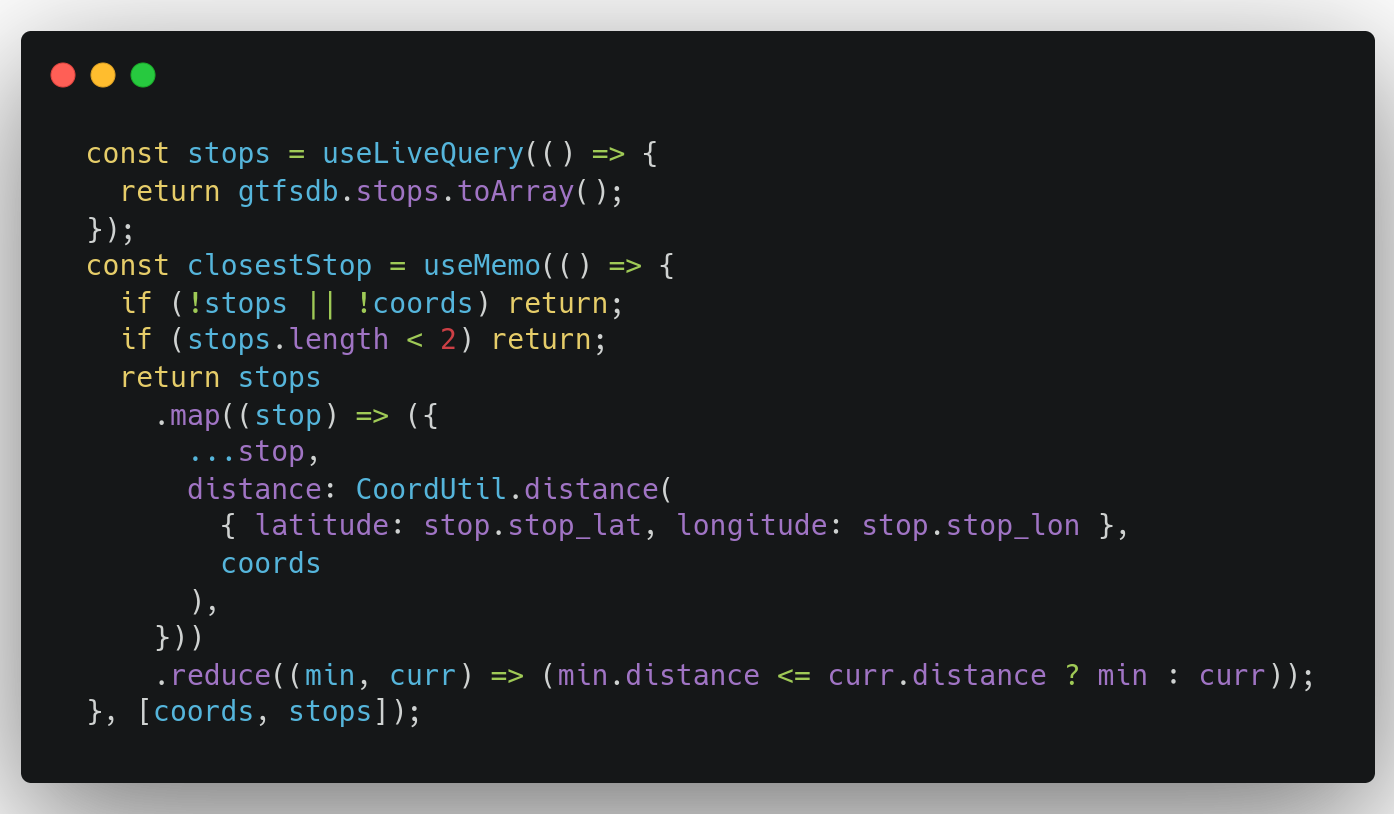
\includegraphics[width=.8\textwidth]{./figures/code/fe_live_queries.png}
    \caption{Frontend: usage of the useLiveQuery hook to retrieve always up-to-date data from IndexedDB.}
    \label{FigFeLiveQueries}
\end{figure}

Figure \ref{FigFeLiveQueries} shows how Dexie's \verb|useLiveQuery| hook is used to find all the stops and then React's \verb|useMemo| hook is used to recalculate the closest station only when either the list of stops or the user coordinates change. This figure exposes the ease with which array manipulation can be performed in JavaScript, using an easy, idiomatic, functional style of fluent function calls.

\begin{figure}[htbp]
    \centering
    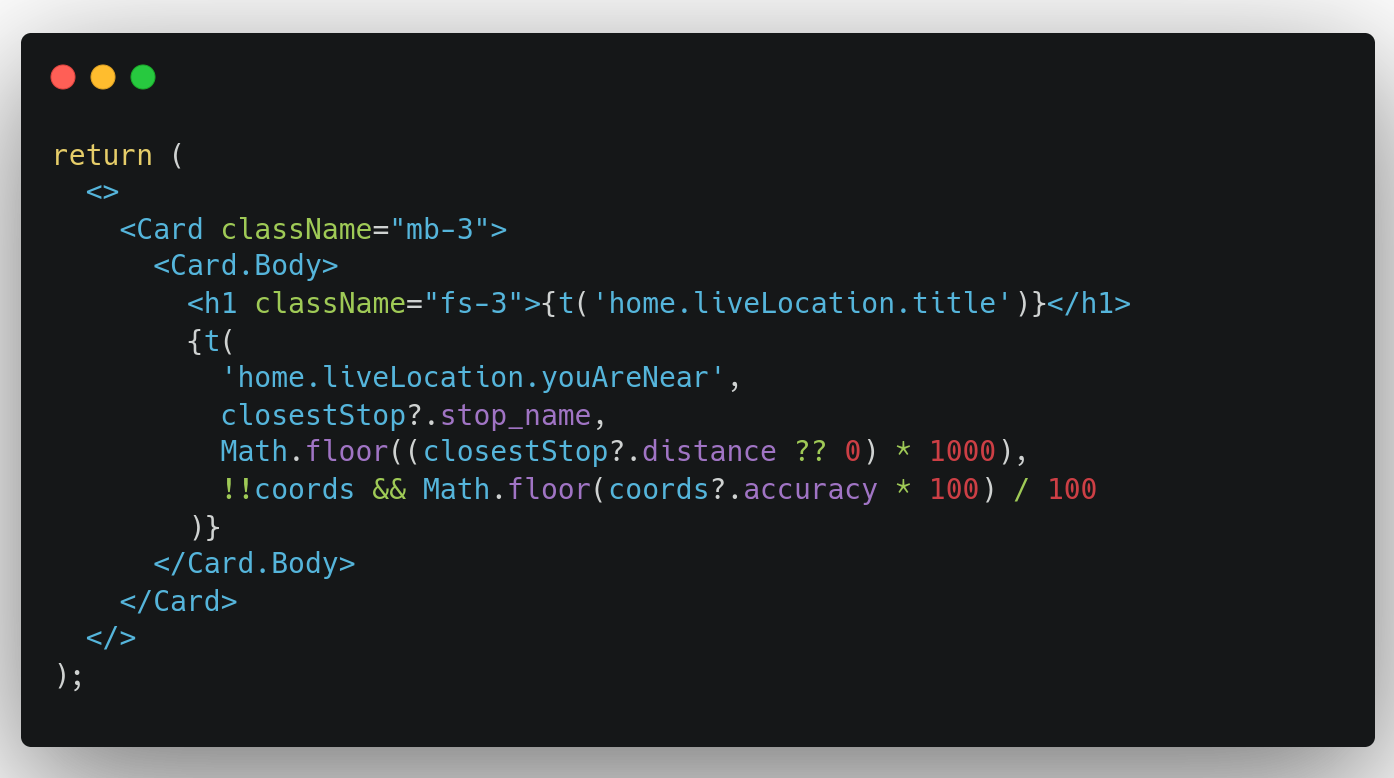
\includegraphics[width=.8\textwidth]{./figures/code/fe_live_jsx.png}
    \caption{Frontend: usage of the translation function in action, while showing, live, the nearest station to the user.}
    \label{FigFeLiveJsx}
\end{figure}

Figure \ref{FigFeLiveJsx} shows the return statement of the component, where the closest stop is displayed to the user by making extensive use of the translation function.

The reactive nature of the calculations really shine during GTFS travel data updates. While IndexedDB does not provide ways of notifying other code when data\-base updates happen, Dexie does keep track of database updates internally and therefore is able to hook into React's reactive system such that it automatically triggers function re-renders whenever relevant updates to the database happen. In this case, it can be seen how the component updates itself automatically when GTFS data is downloaded for the first time.

\subsection{Scanning ticket QR codes}
An important functionality of the application is the ability to scan QR codes located on physical tickets, and automatically figure out the user's current train, and destination.

While the meaning of the QR codes is not documented online, it was possible to reverse-engineer their meaning using a number of train tickets acquired over a period, and try to find out the meaning of each character in the decoded text.

\begin{figure}[htbp]
    \centering
    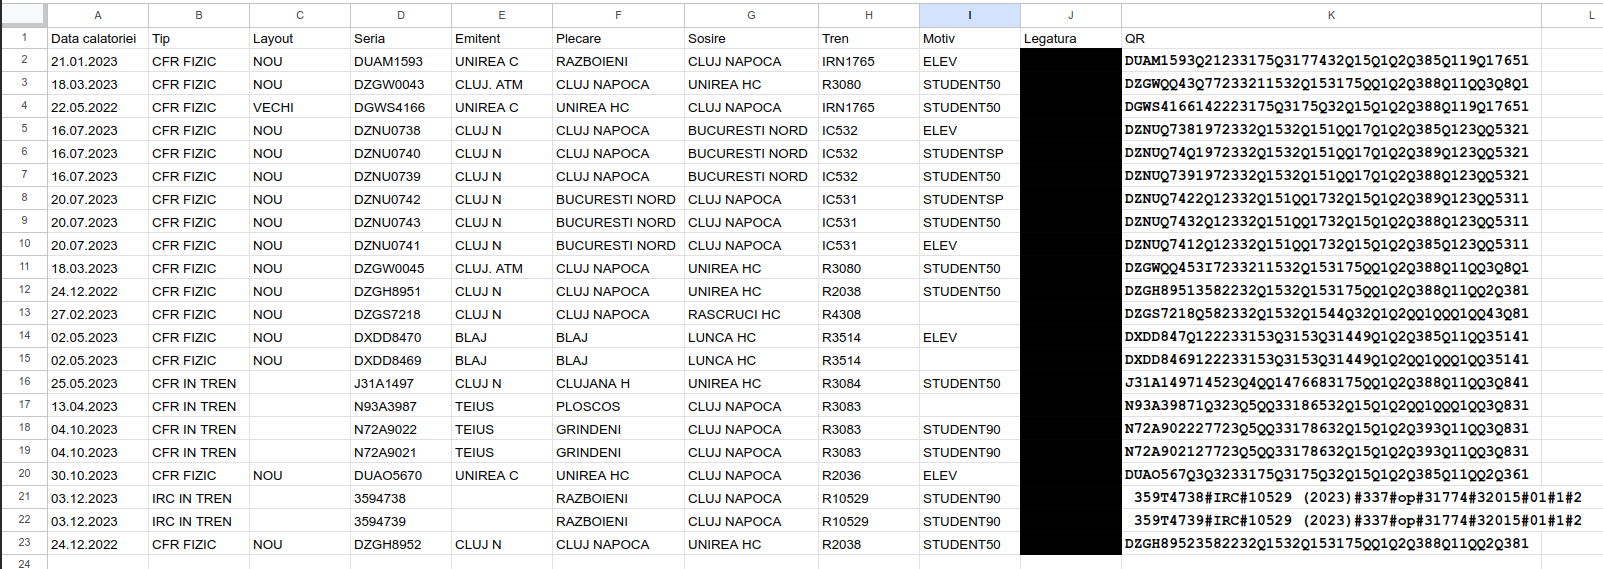
\includegraphics[width=1\textwidth]{./figures/ch4_cfr-tickets.png}
    \caption{Screenshot of the collection of train tickets I have collected for analysis, including two tickets for private operators. Personal information is censored.}
    \label{FigCfrTickets}
\end{figure}

Figure \ref{FigCfrTicketBreakdown} shows a breakdown of the different sections of a decoded ticket QR code. As a first step, we need to convert all \verb|Q| characters from the raw decoded data into zeroes, then we can process the different sections in the manner shown in the figure. It is easy, then, to determine what train the ticket refers to, the departure station, and the ticket's date.

\begin{figure}[htbp]
    \centering
    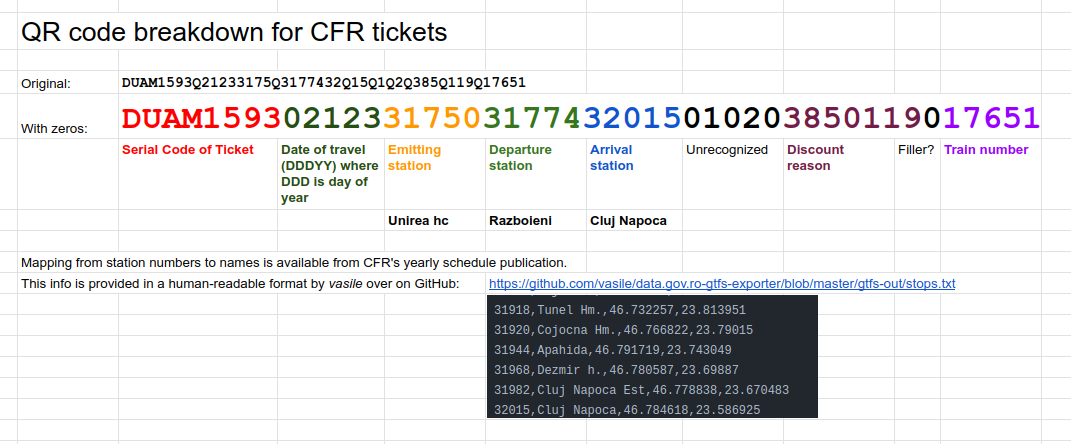
\includegraphics[width=1\textwidth]{./figures/ch4_cfr-ticket-breakdown.png}
    \caption{Breakdown of the QR code data of a CFR ticket.}
    \label{FigCfrTicketBreakdown}
\end{figure}

To integrate QR code scanning into our app, a library has been integrated with React, which performs QR code scanning and returns the raw string data. It is then easy to parse this data according to our rules, and redirect the user to the trip page.

\subsection{Live location: tracking a train}
Tracking a train is the entire point of the application. As a consequence, this feature is the most complex part of it. Let's begin by analyzing the two parts of the Track page: the live location illustration, and the timetable estimations.

\begin{figure}[htbp]
    \centering
    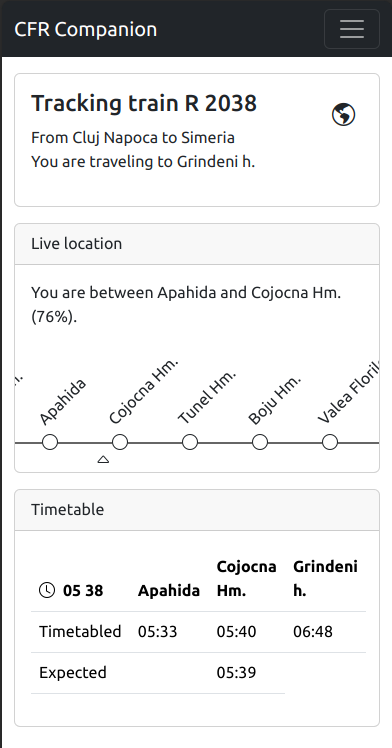
\includegraphics[width=.5\textwidth]{./figures/code/fe_track-all.png}
    \caption{Frontend: the tracking page, in its beautiful entirety.}
    \label{FigFeTrackAll}
\end{figure}

In Figure \ref{FigFeTrackAll}, at the top of the page, you can notice a section titled "Live location". This section displays the closest two stations to the user, and an illustration showing where the user is and what progress towards the next station they've made.

In the same figure, towards the bottom, a table provides arrival estimations for the next station, and the user's destination. The estimation is performed by taking the user's progress along the current leg, and relating it to when they should have departed from the last station, effectively creating an estimation for the train's delay in minutes, in real-time. An example of a two-minute delay is presented in Figure \ref{FigFeTrackWithDelay}.

\begin{figure}[htbp]
    \centering
    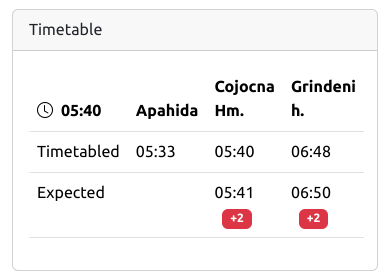
\includegraphics[width=.7\textwidth]{./figures/code/fe_track-with-delay.png}
    \caption{Frontend: how delays appear in the timetable estimations.}
    \label{FigFeTrackWithDelay}
\end{figure}

\subsection{PWA architecture}
Until now, we have described a normal React Single Page Application, that makes use of various browser features such as IndexFigFeTrackWithDelayedDB or live location. However, to turn this application into a PWA, we need to take some additional steps.

Firstly, we need to create an App Manifest. This is a plain JSON file that is used by the browser to determine important metadata about the application. It provides information such as the application name, description, preferred theme color, URL, or scope (path within the origin). This JSON file needs to be publicly accessible, and must be then referenced from the site's HTML using an appropriate \verb|link| tag.

Secondly, possibly the most important step of the process is to create a Service Worker. This service worker takes the form of a JS script that runs in a separate thread from the main page, and has the role of proxying all network requests originating from the main page. It has capability to manage browser caches and inject custom responses even when the network is not available. After creating the worker, it needs to be referenced in the main page's JS code via a Web API, which will enable the browser to register and bootstrap the service worker. This service worker will then persist its state across browser restarts, and across open tabs of the same site.

Thankfully, our bundler Vite provides handy tools to automate this process. Its \verb|vite-plugin-pwa| plugin offers a way of automatically look for the application's assets and create caching strategies for them.

\begin{figure}[htbp]
    \centering
    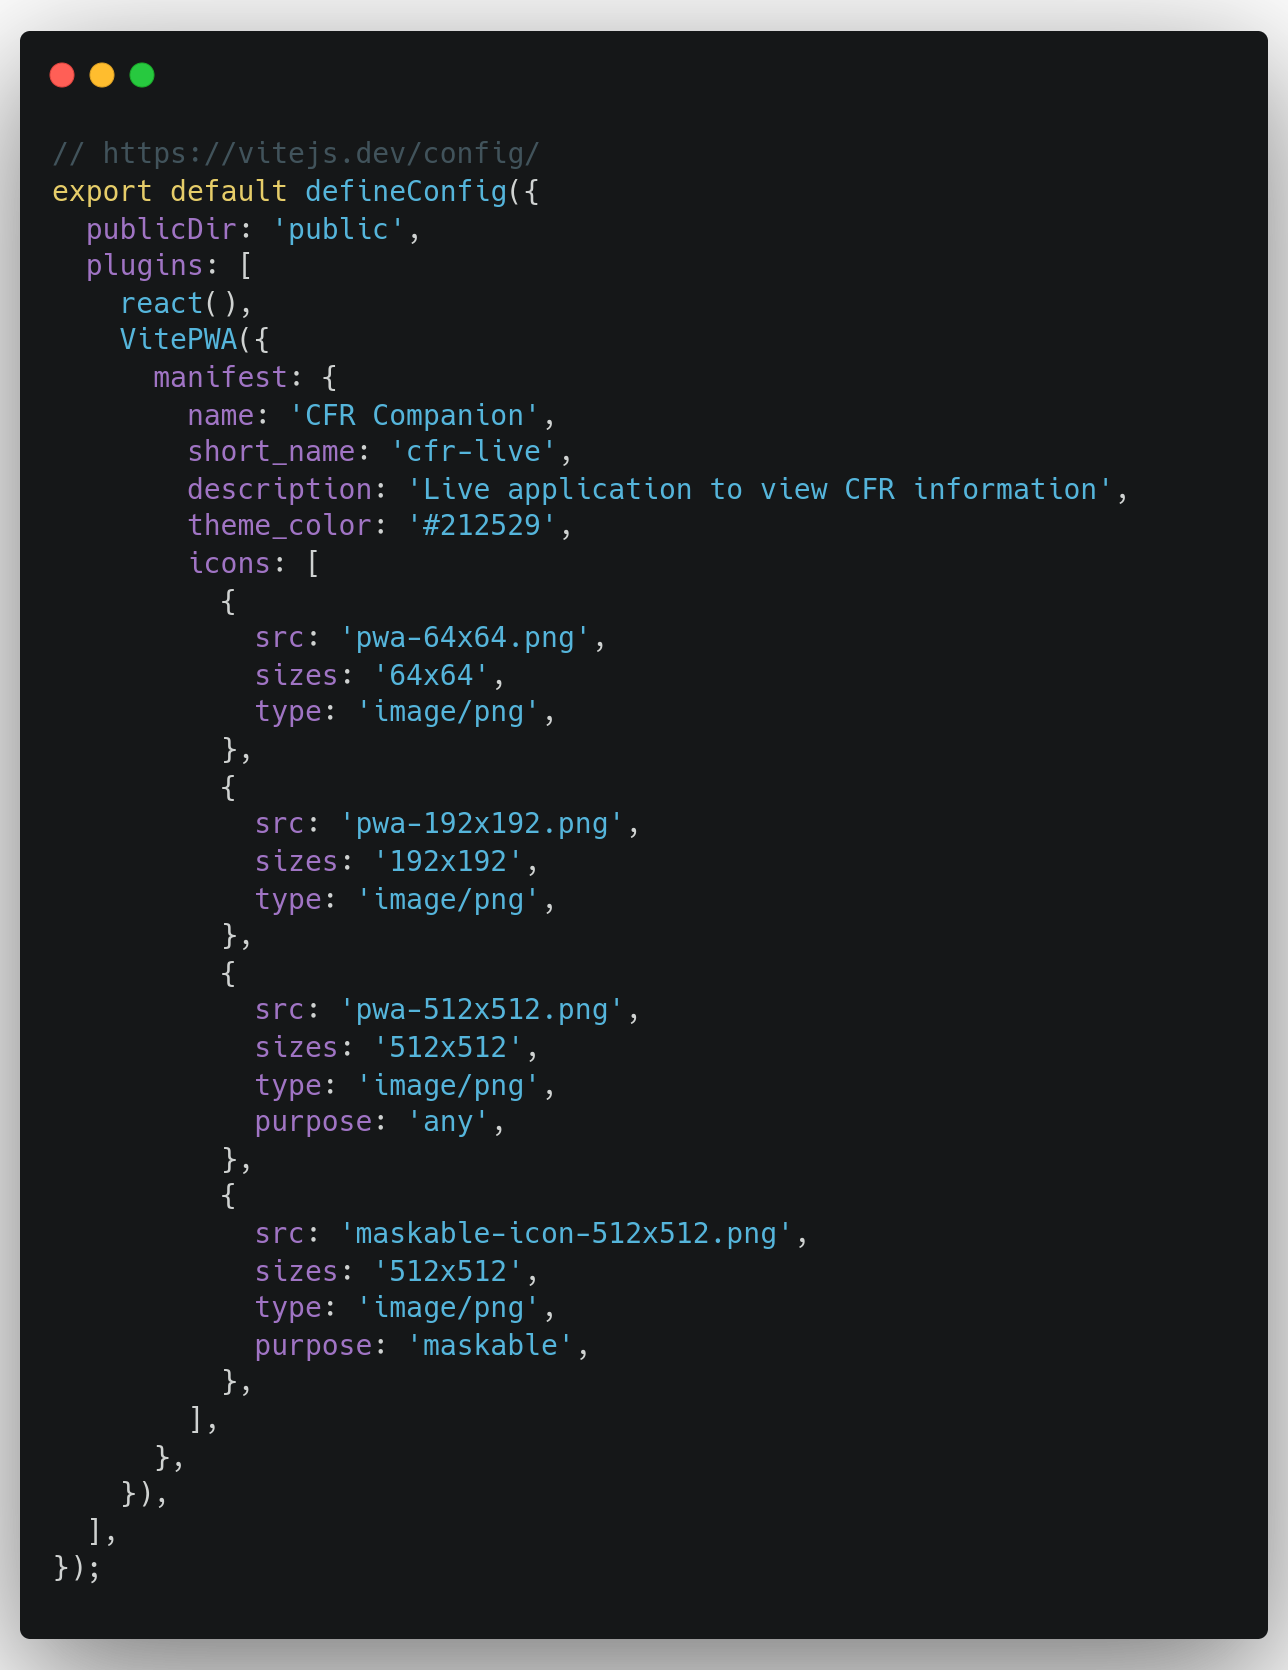
\includegraphics[width=.7\textwidth]{./figures/code/fe_vite-config.png}
    \caption{Frontend: how Vite is configured to produce a PWA-compliant build.}
    \label{FigFeViteConfig}
\end{figure}

Figure \ref{FigFeViteConfig} presents the configuration for the Vite PWA plugin. It takes as parameter only manifest data, which it cannot infer automatically (for obvious reasons). This is all it needs to produce a fully PWA-compliant build, since it can detect application assets (images) automatically.

\subsection{Offline functionality}
An important aspect of the PWA architecture lies in the offline functionality. While Internet connection is required on the first use of the application, it will automatically cache its resources and in the future will work offline out of the box. During this first use the GTFS data is also downloaded, such that train data will also be available offline.

However, certain functionalities require an internet connection to work, namely the authentication system.

To alleviate this issue, the application has code to handle the situation when API calls fail. While failure of API calls does not necessarily mean a lack of internet connection, it does mean that the online features of the application will not work regardless, so it is automatically treated as a "no internet" state.

When the application is not connected, a yellow banner is displayed, alerting the user, and offering the option of retrying. The "retry" button is important, since the app does not have a method of automatically realizing that connectivity is back.

At the same time, functionality that requires internet is hidden, such that the user can not log in anymore (or, if logged in, cannot log out). Additionally, a "no internet" icon is displayed next to the app name.

All this is done to alert the user to their lack of connectivity, but it should be understood that all features that do not explicitly require any API calls will still work, including, notably, usage of itinerary data.

\subsection{Frontend deployment}
The frontend deployment follows a similar constraint set to the ones presented in the counterpart section for the backend (Section \ref{sec:BeDeployment}). Therefore, the deployment flow is very similar.

The difference is notable only in the way the application is served. While the backend runs as a server, a Vite/React build only produces a set of static files, that require a separate server to be served to clients.

To this end, the \textit{nginx} setup on my personal VM helps, and it is configured to statically serve the build artifacts from Vite.

No special configuration is required for the static server to make the application PWA compliant, since the PWA registration is handled in a manner that is transparent to the static server.

\section{Testing}
With a limited scope and feature set, the application is suitable to be manually tested against the requirements outlined in Section \ref{sec:Requirements}.

To be able to test location-related features, I have personally taken builds of the application in various train trips, and noted down any bugs I have encountered. This process definitely helped, and it identified a couple of bugs I couldn't have found otherwise:

\begin{figure}[htbp]
    \centering
    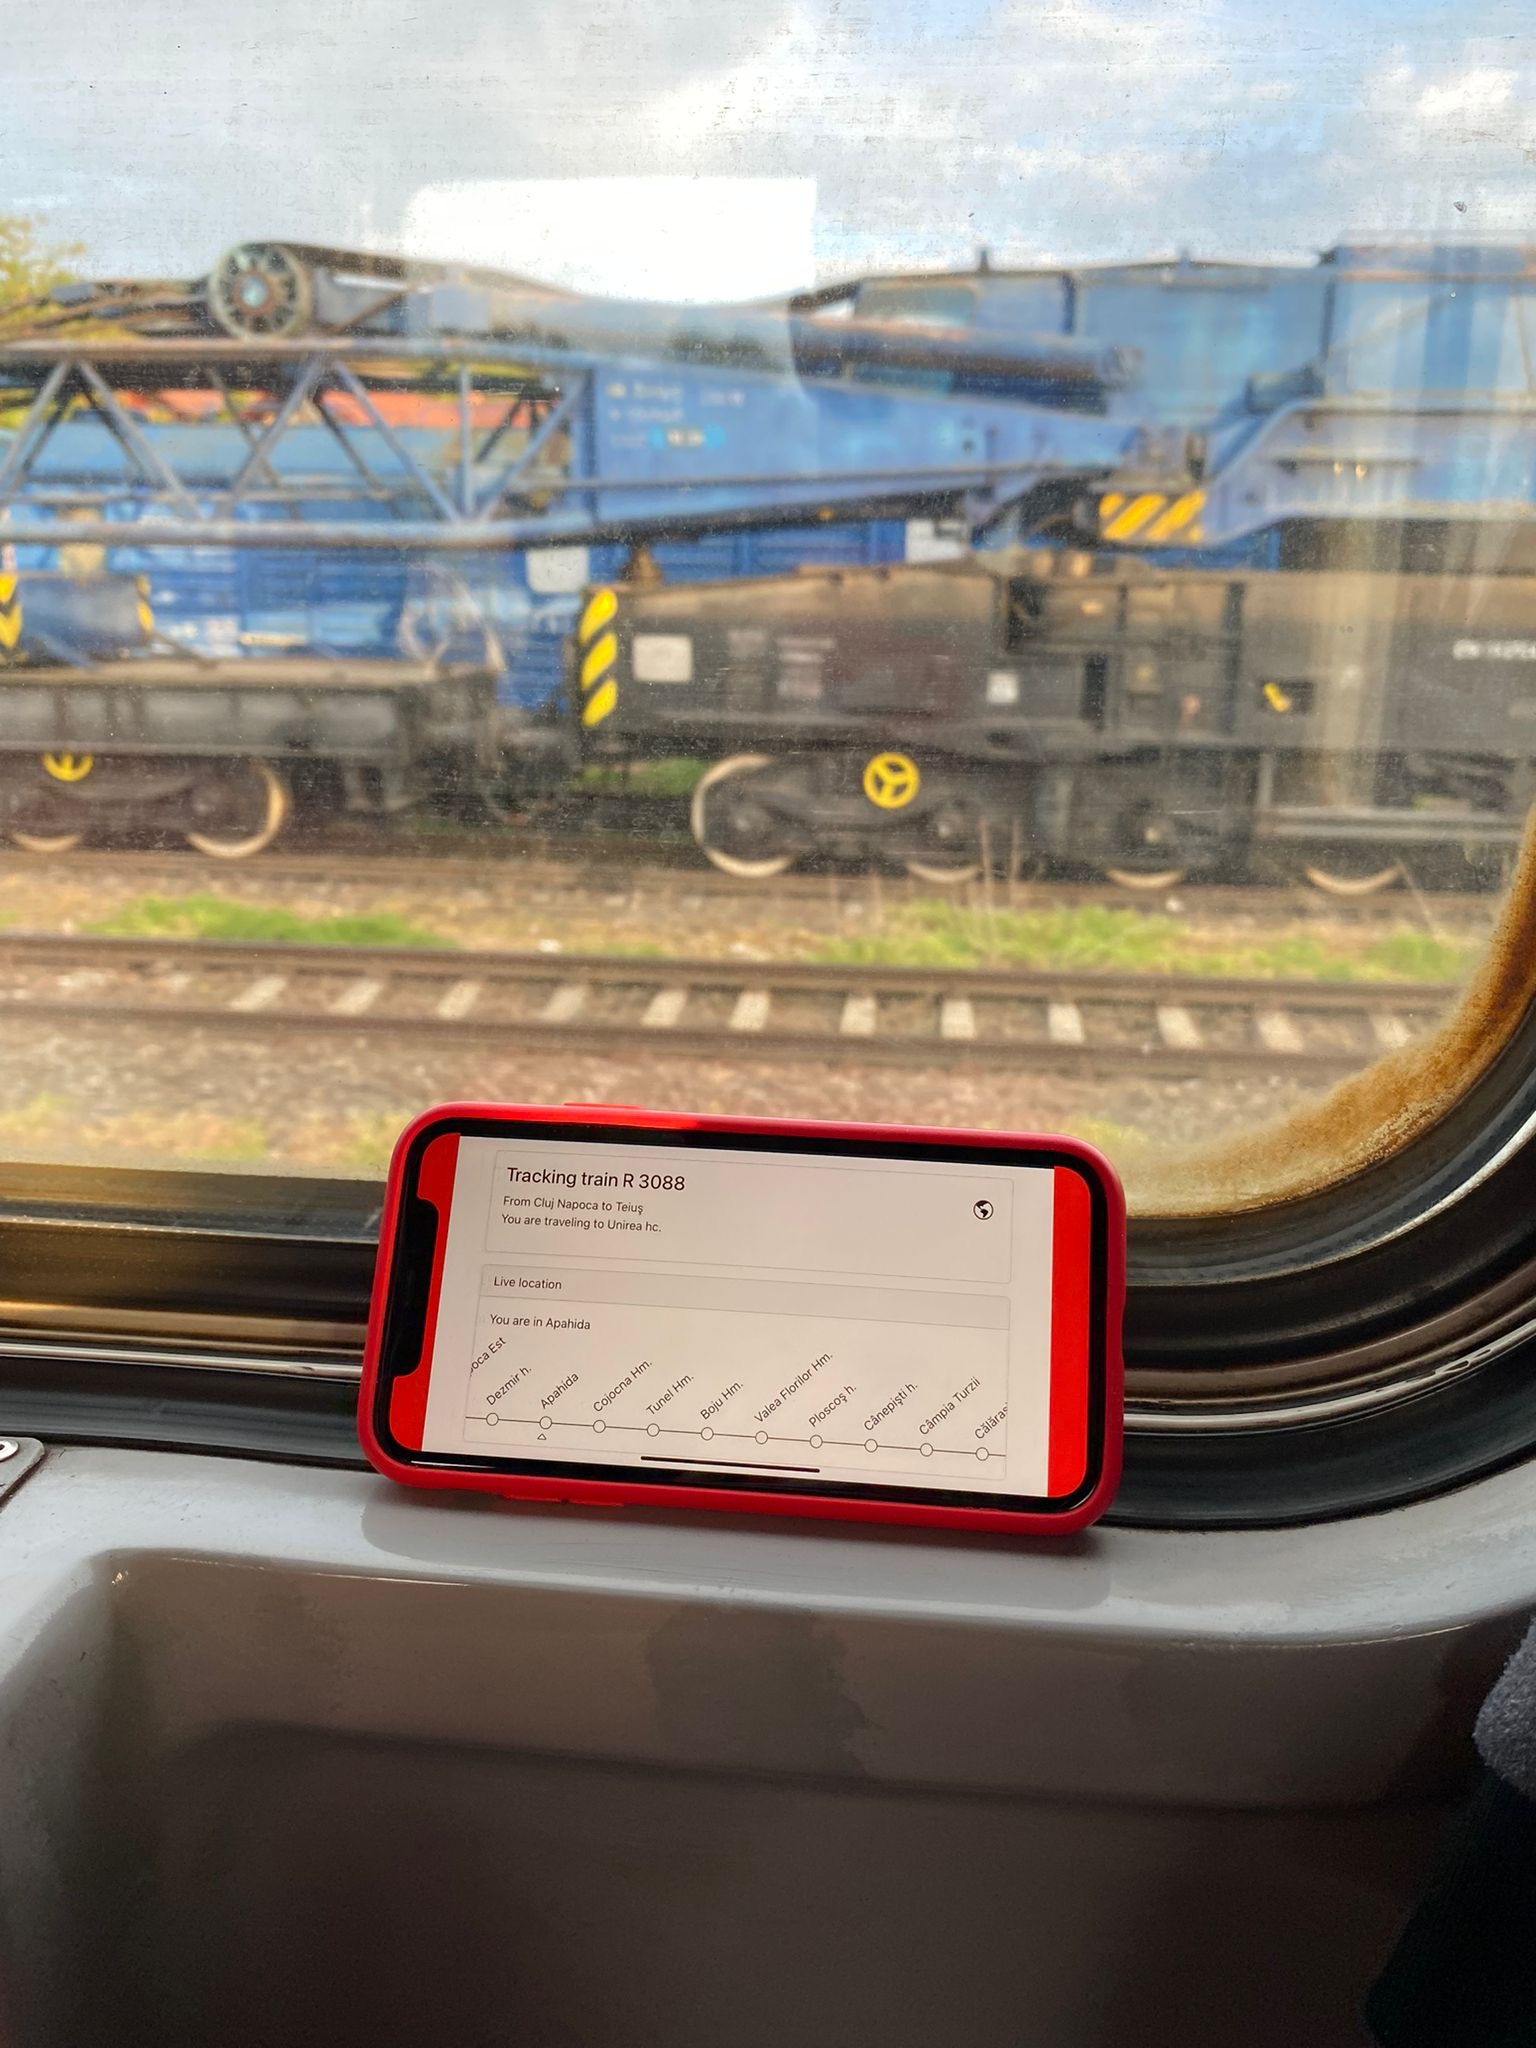
\includegraphics[width=.5\textwidth]{./figures/ch4_manual-testing.JPG}
    \caption{Manual testing of the application, during an actual train trip.}
    \label{FigManualTesting}
\end{figure}

\begin{itemize}
    \item There were instances where the closest two stations did not match up with the stations that you were between. This can happen whenever the station the user has last stopped in is further away than both of the next consecutive stations. To this end, the closest station calculation was modified to better reflect the user's current location relative to the stations.
    \item There were instances where the station coordinates did not match with the real-world location. This is a defect of the GTFS data set, and nothing short of case-by-case correction can be done about it.
    \item A need to automatically scroll the illustration arose from leaving the phone up for extended periods of time.
\end{itemize}

\chapter{Conclusions}

This project was an attempt to prove the usefulness and versatility of Web applications that adhere to the Progressive Web App specification. To this end, I think it was successful, and it shows that a Web application can have the same feature set as a native application, including having the ability to be installed and ran offline, without going through the hassle of developing separate applications for different mobile operating systems.

\section{Potential future work}
The application serves as a useful proof-of-concept of abilities of a PWA application, and it even has potential (in its current form) to be a useful train companion for certain train trips, or for people who travel by train rather rarely.

However, further development opportunities can be identified, some of which are listed below:

\begin{enumerate}
    \item \textbf{Integrating real-time data as received from CFR's official site.} While real-time data from CFR has been considered in this thesis and has been deemed not accurate enough for real-time location tracking, it could prove useful in grounding the application's estimations into the actual reality of the trip.
    \item \textbf{Adding more languages.} While English and Romanian cover a significant part of ridership in Romania, it could be useful to add more languages that tend to other European travelers, such as German or French.
    \item \textbf{Parsing of online tickets.} Online tickets can be purchased for CFR trains and are more convenient than ever before. Although they boast a QR code, the format is not consistent with paper tickets and upon closer inspection does not seem to represent any string data, representing a rather nondescript binary format. However, online tickets come in PDF format, which has potential for different avenues of parsing, in the form of directly looking for text in the PDF file.
    \item \textbf{Parsing of private operator tickets.} Attempting to decode the tickets of private operators could prove as fruitful as decoding CFR physical tickets... or not, but it is an avenue worth exploring.
    \item \textbf{User analytics.} Consenting users could be subjected to event tracking, so as to find out the general usage patterns of features, and make data-backed decisions about the application's interface and functionalities.
\end{enumerate}

% \bibliographystyle{plain}
\bibliography{references}

\end{document}